% Created by tikzDevice version 0.10.1 on 2016-09-05 15:49:48
% !TEX encoding = UTF-8 Unicode
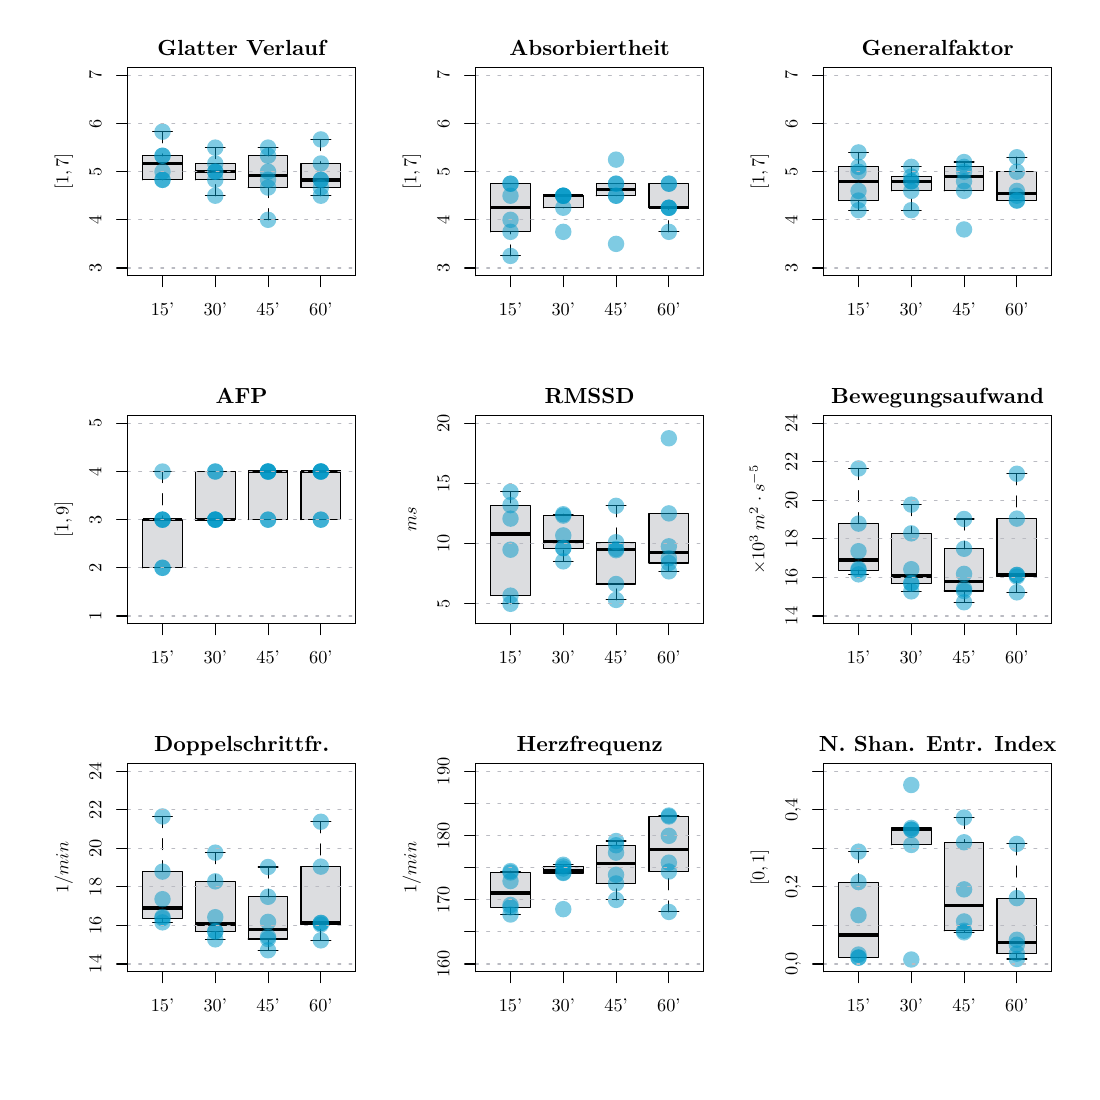
\begin{tikzpicture}[x=1pt,y=1pt]
\definecolor{fillColor}{RGB}{255,255,255}
\path[use as bounding box,fill=fillColor,fill opacity=0.00] (0,0) rectangle (377.25,377.25);
\begin{scope}
\path[clip] ( 36.13,287.63) rectangle (118.52,362.80);
\definecolor{fillColor}{RGB}{186,187,194}

\path[fill=fillColor,fill opacity=0.50] ( 41.57,322.26) --
	( 55.87,322.26) --
	( 55.87,330.96) --
	( 41.57,330.96) --
	cycle;
\definecolor{drawColor}{RGB}{0,0,0}

\path[draw=drawColor,line width= 1.2pt,line join=round] ( 41.57,328.09) -- ( 55.87,328.09);

\path[draw=drawColor,line width= 0.4pt,dash pattern=on 4pt off 4pt ,line join=round,line cap=round] ( 48.72,322.26) -- ( 48.72,322.26);

\path[draw=drawColor,line width= 0.4pt,dash pattern=on 4pt off 4pt ,line join=round,line cap=round] ( 48.72,339.66) -- ( 48.72,330.96);

\path[draw=drawColor,line width= 0.4pt,line join=round,line cap=round] ( 45.15,322.26) -- ( 52.30,322.26);

\path[draw=drawColor,line width= 0.4pt,line join=round,line cap=round] ( 45.15,339.66) -- ( 52.30,339.66);

\path[draw=drawColor,line width= 0.4pt,line join=round,line cap=round] ( 41.57,322.26) --
	( 55.87,322.26) --
	( 55.87,330.96) --
	( 41.57,330.96) --
	( 41.57,322.26);

\path[fill=fillColor,fill opacity=0.50] ( 60.64,322.26) --
	( 74.94,322.26) --
	( 74.94,328.17) --
	( 60.64,328.17) --
	cycle;

\path[draw=drawColor,line width= 1.2pt,line join=round] ( 60.64,325.21) -- ( 74.94,325.21);

\path[draw=drawColor,line width= 0.4pt,dash pattern=on 4pt off 4pt ,line join=round,line cap=round] ( 67.79,316.52) -- ( 67.79,322.26);

\path[draw=drawColor,line width= 0.4pt,dash pattern=on 4pt off 4pt ,line join=round,line cap=round] ( 67.79,333.91) -- ( 67.79,328.17);

\path[draw=drawColor,line width= 0.4pt,line join=round,line cap=round] ( 64.22,316.52) -- ( 71.37,316.52);

\path[draw=drawColor,line width= 0.4pt,line join=round,line cap=round] ( 64.22,333.91) -- ( 71.37,333.91);

\path[draw=drawColor,line width= 0.4pt,line join=round,line cap=round] ( 60.64,322.26) --
	( 74.94,322.26) --
	( 74.94,328.17) --
	( 60.64,328.17) --
	( 60.64,322.26);

\path[fill=fillColor,fill opacity=0.50] ( 79.71,319.47) --
	( 94.02,319.47) --
	( 94.02,330.96) --
	( 79.71,330.96) --
	cycle;

\path[draw=drawColor,line width= 1.2pt,line join=round] ( 79.71,323.74) -- ( 94.02,323.74);

\path[draw=drawColor,line width= 0.4pt,dash pattern=on 4pt off 4pt ,line join=round,line cap=round] ( 86.86,307.82) -- ( 86.86,319.47);

\path[draw=drawColor,line width= 0.4pt,dash pattern=on 4pt off 4pt ,line join=round,line cap=round] ( 86.86,333.91) -- ( 86.86,330.96);

\path[draw=drawColor,line width= 0.4pt,line join=round,line cap=round] ( 83.29,307.82) -- ( 90.44,307.82);

\path[draw=drawColor,line width= 0.4pt,line join=round,line cap=round] ( 83.29,333.91) -- ( 90.44,333.91);

\path[draw=drawColor,line width= 0.4pt,line join=round,line cap=round] ( 79.71,319.47) --
	( 94.02,319.47) --
	( 94.02,330.96) --
	( 79.71,330.96) --
	( 79.71,319.47);

\path[fill=fillColor,fill opacity=0.50] ( 98.78,319.47) --
	(113.09,319.47) --
	(113.09,328.17) --
	( 98.78,328.17) --
	cycle;

\path[draw=drawColor,line width= 1.2pt,line join=round] ( 98.78,322.26) -- (113.09,322.26);

\path[draw=drawColor,line width= 0.4pt,dash pattern=on 4pt off 4pt ,line join=round,line cap=round] (105.94,316.52) -- (105.94,319.47);

\path[draw=drawColor,line width= 0.4pt,dash pattern=on 4pt off 4pt ,line join=round,line cap=round] (105.94,336.87) -- (105.94,328.17);

\path[draw=drawColor,line width= 0.4pt,line join=round,line cap=round] (102.36,316.52) -- (109.51,316.52);

\path[draw=drawColor,line width= 0.4pt,line join=round,line cap=round] (102.36,336.87) -- (109.51,336.87);

\path[draw=drawColor,line width= 0.4pt,line join=round,line cap=round] ( 98.78,319.47) --
	(113.09,319.47) --
	(113.09,328.17) --
	( 98.78,328.17) --
	( 98.78,319.47);
\end{scope}
\begin{scope}
\path[clip] (  0.00,  0.00) rectangle (377.25,377.25);
\definecolor{drawColor}{RGB}{0,0,0}

\path[draw=drawColor,line width= 0.4pt,line join=round,line cap=round] ( 48.72,287.63) -- (105.94,287.63);

\path[draw=drawColor,line width= 0.4pt,line join=round,line cap=round] ( 48.72,287.63) -- ( 48.72,283.67);

\path[draw=drawColor,line width= 0.4pt,line join=round,line cap=round] ( 67.79,287.63) -- ( 67.79,283.67);

\path[draw=drawColor,line width= 0.4pt,line join=round,line cap=round] ( 86.86,287.63) -- ( 86.86,283.67);

\path[draw=drawColor,line width= 0.4pt,line join=round,line cap=round] (105.94,287.63) -- (105.94,283.67);

\node[text=drawColor,anchor=base,inner sep=0pt, outer sep=0pt, scale=  0.66] at ( 48.72,273.38) {15'};

\node[text=drawColor,anchor=base,inner sep=0pt, outer sep=0pt, scale=  0.66] at ( 67.79,273.38) {30'};

\node[text=drawColor,anchor=base,inner sep=0pt, outer sep=0pt, scale=  0.66] at ( 86.86,273.38) {45'};

\node[text=drawColor,anchor=base,inner sep=0pt, outer sep=0pt, scale=  0.66] at (105.94,273.38) {60'};

\path[draw=drawColor,line width= 0.4pt,line join=round,line cap=round] ( 36.13,290.42) -- ( 36.13,360.01);

\path[draw=drawColor,line width= 0.4pt,line join=round,line cap=round] ( 36.13,290.42) -- ( 32.17,290.42);

\path[draw=drawColor,line width= 0.4pt,line join=round,line cap=round] ( 36.13,307.82) -- ( 32.17,307.82);

\path[draw=drawColor,line width= 0.4pt,line join=round,line cap=round] ( 36.13,325.21) -- ( 32.17,325.21);

\path[draw=drawColor,line width= 0.4pt,line join=round,line cap=round] ( 36.13,342.61) -- ( 32.17,342.61);

\path[draw=drawColor,line width= 0.4pt,line join=round,line cap=round] ( 36.13,360.01) -- ( 32.17,360.01);

\node[text=drawColor,rotate= 90.00,anchor=base,inner sep=0pt, outer sep=0pt, scale=  0.66] at ( 26.63,290.42) {3};

\node[text=drawColor,rotate= 90.00,anchor=base,inner sep=0pt, outer sep=0pt, scale=  0.66] at ( 26.63,307.82) {4};

\node[text=drawColor,rotate= 90.00,anchor=base,inner sep=0pt, outer sep=0pt, scale=  0.66] at ( 26.63,325.21) {5};

\node[text=drawColor,rotate= 90.00,anchor=base,inner sep=0pt, outer sep=0pt, scale=  0.66] at ( 26.63,342.61) {6};

\node[text=drawColor,rotate= 90.00,anchor=base,inner sep=0pt, outer sep=0pt, scale=  0.66] at ( 26.63,360.01) {7};
\end{scope}
\begin{scope}
\path[clip] (  0.00,251.50) rectangle (125.75,377.25);
\definecolor{drawColor}{RGB}{0,0,0}

\node[text=drawColor,anchor=base,inner sep=0pt, outer sep=0pt, scale=  0.79] at ( 77.33,367.29) {\bfseries Glatter Verlauf};

\node[text=drawColor,rotate= 90.00,anchor=base,inner sep=0pt, outer sep=0pt, scale=  0.66] at ( 14.75,325.21) {$[1, 7]$};
\end{scope}
\begin{scope}
\path[clip] (  0.00,  0.00) rectangle (377.25,377.25);
\definecolor{drawColor}{RGB}{0,0,0}

\path[draw=drawColor,line width= 0.4pt,line join=round,line cap=round] ( 36.13,287.63) --
	(118.52,287.63) --
	(118.52,362.80) --
	( 36.13,362.80) --
	( 36.13,287.63);
\end{scope}
\begin{scope}
\path[clip] ( 36.13,287.63) rectangle (118.52,362.80);
\definecolor{fillColor}{RGB}{0,152,199}

\path[fill=fillColor,fill opacity=0.50] ( 48.72,325.21) circle (  2.97);

\path[fill=fillColor,fill opacity=0.50] ( 67.79,322.26) circle (  2.97);

\path[fill=fillColor,fill opacity=0.50] ( 86.86,319.47) circle (  2.97);

\path[fill=fillColor,fill opacity=0.50] (105.94,319.47) circle (  2.97);

\path[fill=fillColor,fill opacity=0.50] ( 48.72,322.26) circle (  2.97);

\path[fill=fillColor,fill opacity=0.50] ( 67.79,325.21) circle (  2.97);

\path[fill=fillColor,fill opacity=0.50] ( 86.86,325.21) circle (  2.97);

\path[fill=fillColor,fill opacity=0.50] (105.94,322.26) circle (  2.97);

\path[fill=fillColor,fill opacity=0.50] ( 48.72,322.26) circle (  2.97);

\path[fill=fillColor,fill opacity=0.50] ( 67.79,316.52) circle (  2.97);

\path[fill=fillColor,fill opacity=0.50] ( 86.86,307.82) circle (  2.97);

\path[fill=fillColor,fill opacity=0.50] (105.94,316.52) circle (  2.97);

\path[fill=fillColor,fill opacity=0.50] ( 48.72,330.96) circle (  2.97);

\path[fill=fillColor,fill opacity=0.50] ( 67.79,325.21) circle (  2.97);

\path[fill=fillColor,fill opacity=0.50] ( 86.86,333.91) circle (  2.97);

\path[fill=fillColor,fill opacity=0.50] (105.94,328.17) circle (  2.97);

\path[fill=fillColor,fill opacity=0.50] ( 48.72,330.96) circle (  2.97);

\path[fill=fillColor,fill opacity=0.50] ( 67.79,328.17) circle (  2.97);

\path[fill=fillColor,fill opacity=0.50] ( 86.86,330.96) circle (  2.97);

\path[fill=fillColor,fill opacity=0.50] (105.94,336.87) circle (  2.97);

\path[fill=fillColor,fill opacity=0.50] ( 48.72,339.66) circle (  2.97);

\path[fill=fillColor,fill opacity=0.50] ( 67.79,333.91) circle (  2.97);

\path[fill=fillColor,fill opacity=0.50] ( 86.86,322.26) circle (  2.97);

\path[fill=fillColor,fill opacity=0.50] (105.94,322.26) circle (  2.97);
\definecolor{drawColor}{RGB}{186,187,194}

\path[draw=drawColor,line width= 0.4pt,dash pattern=on 1pt off 3pt ,line join=round,line cap=round] ( 36.13,290.42) -- (118.52,290.42);

\path[draw=drawColor,line width= 0.4pt,dash pattern=on 1pt off 3pt ,line join=round,line cap=round] ( 36.13,307.82) -- (118.52,307.82);

\path[draw=drawColor,line width= 0.4pt,dash pattern=on 1pt off 3pt ,line join=round,line cap=round] ( 36.13,325.21) -- (118.52,325.21);

\path[draw=drawColor,line width= 0.4pt,dash pattern=on 1pt off 3pt ,line join=round,line cap=round] ( 36.13,342.61) -- (118.52,342.61);

\path[draw=drawColor,line width= 0.4pt,dash pattern=on 1pt off 3pt ,line join=round,line cap=round] ( 36.13,360.01) -- (118.52,360.01);
\end{scope}
\begin{scope}
\path[clip] (  0.00,  0.00) rectangle (377.25,377.25);
\definecolor{drawColor}{RGB}{0,0,0}

\path[draw=drawColor,line width= 0.4pt,line join=round,line cap=round] ( 36.13,287.63) --
	(118.52,287.63) --
	(118.52,362.80) --
	( 36.13,362.80) --
	( 36.13,287.63);
\end{scope}
\begin{scope}
\path[clip] (161.88,287.63) rectangle (244.27,362.80);
\definecolor{fillColor}{RGB}{186,187,194}

\path[fill=fillColor,fill opacity=0.50] (167.32,303.47) --
	(181.62,303.47) --
	(181.62,320.87) --
	(167.32,320.87) --
	cycle;
\definecolor{drawColor}{RGB}{0,0,0}

\path[draw=drawColor,line width= 1.2pt,line join=round] (167.32,312.17) -- (181.62,312.17);

\path[draw=drawColor,line width= 0.4pt,dash pattern=on 4pt off 4pt ,line join=round,line cap=round] (174.47,294.77) -- (174.47,303.47);

\path[draw=drawColor,line width= 0.4pt,dash pattern=on 4pt off 4pt ,line join=round,line cap=round] (174.47,320.87) -- (174.47,320.87);

\path[draw=drawColor,line width= 0.4pt,line join=round,line cap=round] (170.90,294.77) -- (178.05,294.77);

\path[draw=drawColor,line width= 0.4pt,line join=round,line cap=round] (170.90,320.87) -- (178.05,320.87);

\path[draw=drawColor,line width= 0.4pt,line join=round,line cap=round] (167.32,303.47) --
	(181.62,303.47) --
	(181.62,320.87) --
	(167.32,320.87) --
	(167.32,303.47);

\path[fill=fillColor,fill opacity=0.50] (186.39,312.17) --
	(200.69,312.17) --
	(200.69,316.52) --
	(186.39,316.52) --
	cycle;

\path[draw=drawColor,line width= 1.2pt,line join=round] (186.39,316.52) -- (200.69,316.52);

\path[draw=drawColor,line width= 0.4pt,dash pattern=on 4pt off 4pt ,line join=round,line cap=round] (193.54,312.17) -- (193.54,312.17);

\path[draw=drawColor,line width= 0.4pt,dash pattern=on 4pt off 4pt ,line join=round,line cap=round] (193.54,316.52) -- (193.54,316.52);

\path[draw=drawColor,line width= 0.4pt,line join=round,line cap=round] (189.97,312.17) -- (197.12,312.17);

\path[draw=drawColor,line width= 0.4pt,line join=round,line cap=round] (189.97,316.52) -- (197.12,316.52);

\path[draw=drawColor,line width= 0.4pt,line join=round,line cap=round] (186.39,312.17) --
	(200.69,312.17) --
	(200.69,316.52) --
	(186.39,316.52) --
	(186.39,312.17);

\path[fill=fillColor,fill opacity=0.50] (205.46,316.52) --
	(219.77,316.52) --
	(219.77,320.87) --
	(205.46,320.87) --
	cycle;

\path[draw=drawColor,line width= 1.2pt,line join=round] (205.46,318.69) -- (219.77,318.69);

\path[draw=drawColor,line width= 0.4pt,dash pattern=on 4pt off 4pt ,line join=round,line cap=round] (212.61,316.52) -- (212.61,316.52);

\path[draw=drawColor,line width= 0.4pt,dash pattern=on 4pt off 4pt ,line join=round,line cap=round] (212.61,320.87) -- (212.61,320.87);

\path[draw=drawColor,line width= 0.4pt,line join=round,line cap=round] (209.04,316.52) -- (216.19,316.52);

\path[draw=drawColor,line width= 0.4pt,line join=round,line cap=round] (209.04,320.87) -- (216.19,320.87);

\path[draw=drawColor,line width= 0.4pt,line join=round,line cap=round] (205.46,316.52) --
	(219.77,316.52) --
	(219.77,320.87) --
	(205.46,320.87) --
	(205.46,316.52);

\path[fill=fillColor,fill opacity=0.50] (224.53,312.17) --
	(238.84,312.17) --
	(238.84,320.87) --
	(224.53,320.87) --
	cycle;

\path[draw=drawColor,line width= 1.2pt,line join=round] (224.53,312.17) -- (238.84,312.17);

\path[draw=drawColor,line width= 0.4pt,dash pattern=on 4pt off 4pt ,line join=round,line cap=round] (231.69,303.47) -- (231.69,312.17);

\path[draw=drawColor,line width= 0.4pt,dash pattern=on 4pt off 4pt ,line join=round,line cap=round] (231.69,320.87) -- (231.69,320.87);

\path[draw=drawColor,line width= 0.4pt,line join=round,line cap=round] (228.11,303.47) -- (235.26,303.47);

\path[draw=drawColor,line width= 0.4pt,line join=round,line cap=round] (228.11,320.87) -- (235.26,320.87);

\path[draw=drawColor,line width= 0.4pt,line join=round,line cap=round] (224.53,312.17) --
	(238.84,312.17) --
	(238.84,320.87) --
	(224.53,320.87) --
	(224.53,312.17);
\end{scope}
\begin{scope}
\path[clip] (  0.00,  0.00) rectangle (377.25,377.25);
\definecolor{drawColor}{RGB}{0,0,0}

\path[draw=drawColor,line width= 0.4pt,line join=round,line cap=round] (174.47,287.63) -- (231.69,287.63);

\path[draw=drawColor,line width= 0.4pt,line join=round,line cap=round] (174.47,287.63) -- (174.47,283.67);

\path[draw=drawColor,line width= 0.4pt,line join=round,line cap=round] (193.54,287.63) -- (193.54,283.67);

\path[draw=drawColor,line width= 0.4pt,line join=round,line cap=round] (212.61,287.63) -- (212.61,283.67);

\path[draw=drawColor,line width= 0.4pt,line join=round,line cap=round] (231.69,287.63) -- (231.69,283.67);

\node[text=drawColor,anchor=base,inner sep=0pt, outer sep=0pt, scale=  0.66] at (174.47,273.38) {15'};

\node[text=drawColor,anchor=base,inner sep=0pt, outer sep=0pt, scale=  0.66] at (193.54,273.38) {30'};

\node[text=drawColor,anchor=base,inner sep=0pt, outer sep=0pt, scale=  0.66] at (212.61,273.38) {45'};

\node[text=drawColor,anchor=base,inner sep=0pt, outer sep=0pt, scale=  0.66] at (231.69,273.38) {60'};

\path[draw=drawColor,line width= 0.4pt,line join=round,line cap=round] (161.88,290.42) -- (161.88,360.01);

\path[draw=drawColor,line width= 0.4pt,line join=round,line cap=round] (161.88,290.42) -- (157.92,290.42);

\path[draw=drawColor,line width= 0.4pt,line join=round,line cap=round] (161.88,307.82) -- (157.92,307.82);

\path[draw=drawColor,line width= 0.4pt,line join=round,line cap=round] (161.88,325.21) -- (157.92,325.21);

\path[draw=drawColor,line width= 0.4pt,line join=round,line cap=round] (161.88,342.61) -- (157.92,342.61);

\path[draw=drawColor,line width= 0.4pt,line join=round,line cap=round] (161.88,360.01) -- (157.92,360.01);

\node[text=drawColor,rotate= 90.00,anchor=base,inner sep=0pt, outer sep=0pt, scale=  0.66] at (152.38,290.42) {3};

\node[text=drawColor,rotate= 90.00,anchor=base,inner sep=0pt, outer sep=0pt, scale=  0.66] at (152.38,307.82) {4};

\node[text=drawColor,rotate= 90.00,anchor=base,inner sep=0pt, outer sep=0pt, scale=  0.66] at (152.38,325.21) {5};

\node[text=drawColor,rotate= 90.00,anchor=base,inner sep=0pt, outer sep=0pt, scale=  0.66] at (152.38,342.61) {6};

\node[text=drawColor,rotate= 90.00,anchor=base,inner sep=0pt, outer sep=0pt, scale=  0.66] at (152.38,360.01) {7};
\end{scope}
\begin{scope}
\path[clip] (125.75,251.50) rectangle (251.50,377.25);
\definecolor{drawColor}{RGB}{0,0,0}

\node[text=drawColor,anchor=base,inner sep=0pt, outer sep=0pt, scale=  0.79] at (203.08,367.29) {\bfseries Absorbiertheit};

\node[text=drawColor,rotate= 90.00,anchor=base,inner sep=0pt, outer sep=0pt, scale=  0.66] at (140.50,325.21) {$[1, 7]$};
\end{scope}
\begin{scope}
\path[clip] (  0.00,  0.00) rectangle (377.25,377.25);
\definecolor{drawColor}{RGB}{0,0,0}

\path[draw=drawColor,line width= 0.4pt,line join=round,line cap=round] (161.88,287.63) --
	(244.27,287.63) --
	(244.27,362.80) --
	(161.88,362.80) --
	(161.88,287.63);
\end{scope}
\begin{scope}
\path[clip] (161.88,287.63) rectangle (244.27,362.80);
\definecolor{fillColor}{RGB}{0,152,199}

\path[fill=fillColor,fill opacity=0.50] (174.47,307.82) circle (  2.97);

\path[fill=fillColor,fill opacity=0.50] (193.54,312.17) circle (  2.97);

\path[fill=fillColor,fill opacity=0.50] (212.61,316.52) circle (  2.97);

\path[fill=fillColor,fill opacity=0.50] (231.69,312.17) circle (  2.97);

\path[fill=fillColor,fill opacity=0.50] (174.47,294.77) circle (  2.97);

\path[fill=fillColor,fill opacity=0.50] (193.54,316.52) circle (  2.97);

\path[fill=fillColor,fill opacity=0.50] (212.61,316.52) circle (  2.97);

\path[fill=fillColor,fill opacity=0.50] (231.69,312.17) circle (  2.97);

\path[fill=fillColor,fill opacity=0.50] (174.47,303.47) circle (  2.97);

\path[fill=fillColor,fill opacity=0.50] (193.54,303.47) circle (  2.97);

\path[fill=fillColor,fill opacity=0.50] (212.61,299.12) circle (  2.97);

\path[fill=fillColor,fill opacity=0.50] (231.69,312.17) circle (  2.97);

\path[fill=fillColor,fill opacity=0.50] (174.47,316.52) circle (  2.97);

\path[fill=fillColor,fill opacity=0.50] (193.54,316.52) circle (  2.97);

\path[fill=fillColor,fill opacity=0.50] (212.61,320.87) circle (  2.97);

\path[fill=fillColor,fill opacity=0.50] (231.69,320.87) circle (  2.97);

\path[fill=fillColor,fill opacity=0.50] (174.47,320.87) circle (  2.97);

\path[fill=fillColor,fill opacity=0.50] (193.54,316.52) circle (  2.97);

\path[fill=fillColor,fill opacity=0.50] (212.61,320.87) circle (  2.97);

\path[fill=fillColor,fill opacity=0.50] (231.69,320.87) circle (  2.97);

\path[fill=fillColor,fill opacity=0.50] (174.47,320.87) circle (  2.97);

\path[fill=fillColor,fill opacity=0.50] (193.54,316.52) circle (  2.97);

\path[fill=fillColor,fill opacity=0.50] (212.61,329.56) circle (  2.97);

\path[fill=fillColor,fill opacity=0.50] (231.69,303.47) circle (  2.97);
\definecolor{drawColor}{RGB}{186,187,194}

\path[draw=drawColor,line width= 0.4pt,dash pattern=on 1pt off 3pt ,line join=round,line cap=round] (161.88,290.42) -- (244.27,290.42);

\path[draw=drawColor,line width= 0.4pt,dash pattern=on 1pt off 3pt ,line join=round,line cap=round] (161.88,307.82) -- (244.27,307.82);

\path[draw=drawColor,line width= 0.4pt,dash pattern=on 1pt off 3pt ,line join=round,line cap=round] (161.88,325.21) -- (244.27,325.21);

\path[draw=drawColor,line width= 0.4pt,dash pattern=on 1pt off 3pt ,line join=round,line cap=round] (161.88,342.61) -- (244.27,342.61);

\path[draw=drawColor,line width= 0.4pt,dash pattern=on 1pt off 3pt ,line join=round,line cap=round] (161.88,360.01) -- (244.27,360.01);
\end{scope}
\begin{scope}
\path[clip] (  0.00,  0.00) rectangle (377.25,377.25);
\definecolor{drawColor}{RGB}{0,0,0}

\path[draw=drawColor,line width= 0.4pt,line join=round,line cap=round] (161.88,287.63) --
	(244.27,287.63) --
	(244.27,362.80) --
	(161.88,362.80) --
	(161.88,287.63);
\end{scope}
\begin{scope}
\path[clip] (287.63,287.63) rectangle (370.02,362.80);
\definecolor{fillColor}{RGB}{186,187,194}

\path[fill=fillColor,fill opacity=0.50] (293.07,314.78) --
	(307.37,314.78) --
	(307.37,326.95) --
	(293.07,326.95) --
	cycle;
\definecolor{drawColor}{RGB}{0,0,0}

\path[draw=drawColor,line width= 1.2pt,line join=round] (293.07,321.74) -- (307.37,321.74);

\path[draw=drawColor,line width= 0.4pt,dash pattern=on 4pt off 4pt ,line join=round,line cap=round] (300.22,311.30) -- (300.22,314.78);

\path[draw=drawColor,line width= 0.4pt,dash pattern=on 4pt off 4pt ,line join=round,line cap=round] (300.22,332.17) -- (300.22,326.95);

\path[draw=drawColor,line width= 0.4pt,line join=round,line cap=round] (296.65,311.30) -- (303.80,311.30);

\path[draw=drawColor,line width= 0.4pt,line join=round,line cap=round] (296.65,332.17) -- (303.80,332.17);

\path[draw=drawColor,line width= 0.4pt,line join=round,line cap=round] (293.07,314.78) --
	(307.37,314.78) --
	(307.37,326.95) --
	(293.07,326.95) --
	(293.07,314.78);

\path[fill=fillColor,fill opacity=0.50] (312.14,318.26) --
	(326.44,318.26) --
	(326.44,323.48) --
	(312.14,323.48) --
	cycle;

\path[draw=drawColor,line width= 1.2pt,line join=round] (312.14,321.74) -- (326.44,321.74);

\path[draw=drawColor,line width= 0.4pt,dash pattern=on 4pt off 4pt ,line join=round,line cap=round] (319.29,311.30) -- (319.29,318.26);

\path[draw=drawColor,line width= 0.4pt,dash pattern=on 4pt off 4pt ,line join=round,line cap=round] (319.29,326.95) -- (319.29,323.48);

\path[draw=drawColor,line width= 0.4pt,line join=round,line cap=round] (315.72,311.30) -- (322.87,311.30);

\path[draw=drawColor,line width= 0.4pt,line join=round,line cap=round] (315.72,326.95) -- (322.87,326.95);

\path[draw=drawColor,line width= 0.4pt,line join=round,line cap=round] (312.14,318.26) --
	(326.44,318.26) --
	(326.44,323.48) --
	(312.14,323.48) --
	(312.14,318.26);

\path[fill=fillColor,fill opacity=0.50] (331.21,318.26) --
	(345.52,318.26) --
	(345.52,326.95) --
	(331.21,326.95) --
	cycle;

\path[draw=drawColor,line width= 1.2pt,line join=round] (331.21,323.48) -- (345.52,323.48);

\path[draw=drawColor,line width= 0.4pt,dash pattern=on 4pt off 4pt ,line join=round,line cap=round] (338.36,318.26) -- (338.36,318.26);

\path[draw=drawColor,line width= 0.4pt,dash pattern=on 4pt off 4pt ,line join=round,line cap=round] (338.36,328.69) -- (338.36,326.95);

\path[draw=drawColor,line width= 0.4pt,line join=round,line cap=round] (334.79,318.26) -- (341.94,318.26);

\path[draw=drawColor,line width= 0.4pt,line join=round,line cap=round] (334.79,328.69) -- (341.94,328.69);

\path[draw=drawColor,line width= 0.4pt,line join=round,line cap=round] (331.21,318.26) --
	(345.52,318.26) --
	(345.52,326.95) --
	(331.21,326.95) --
	(331.21,318.26);

\path[fill=fillColor,fill opacity=0.50] (350.28,314.78) --
	(364.59,314.78) --
	(364.59,325.21) --
	(350.28,325.21) --
	cycle;

\path[draw=drawColor,line width= 1.2pt,line join=round] (350.28,317.39) -- (364.59,317.39);

\path[draw=drawColor,line width= 0.4pt,dash pattern=on 4pt off 4pt ,line join=round,line cap=round] (357.44,314.78) -- (357.44,314.78);

\path[draw=drawColor,line width= 0.4pt,dash pattern=on 4pt off 4pt ,line join=round,line cap=round] (357.44,330.43) -- (357.44,325.21);

\path[draw=drawColor,line width= 0.4pt,line join=round,line cap=round] (353.86,314.78) -- (361.01,314.78);

\path[draw=drawColor,line width= 0.4pt,line join=round,line cap=round] (353.86,330.43) -- (361.01,330.43);

\path[draw=drawColor,line width= 0.4pt,line join=round,line cap=round] (350.28,314.78) --
	(364.59,314.78) --
	(364.59,325.21) --
	(350.28,325.21) --
	(350.28,314.78);
\end{scope}
\begin{scope}
\path[clip] (  0.00,  0.00) rectangle (377.25,377.25);
\definecolor{drawColor}{RGB}{0,0,0}

\path[draw=drawColor,line width= 0.4pt,line join=round,line cap=round] (300.22,287.63) -- (357.44,287.63);

\path[draw=drawColor,line width= 0.4pt,line join=round,line cap=round] (300.22,287.63) -- (300.22,283.67);

\path[draw=drawColor,line width= 0.4pt,line join=round,line cap=round] (319.29,287.63) -- (319.29,283.67);

\path[draw=drawColor,line width= 0.4pt,line join=round,line cap=round] (338.36,287.63) -- (338.36,283.67);

\path[draw=drawColor,line width= 0.4pt,line join=round,line cap=round] (357.44,287.63) -- (357.44,283.67);

\node[text=drawColor,anchor=base,inner sep=0pt, outer sep=0pt, scale=  0.66] at (300.22,273.38) {15'};

\node[text=drawColor,anchor=base,inner sep=0pt, outer sep=0pt, scale=  0.66] at (319.29,273.38) {30'};

\node[text=drawColor,anchor=base,inner sep=0pt, outer sep=0pt, scale=  0.66] at (338.36,273.38) {45'};

\node[text=drawColor,anchor=base,inner sep=0pt, outer sep=0pt, scale=  0.66] at (357.44,273.38) {60'};

\path[draw=drawColor,line width= 0.4pt,line join=round,line cap=round] (287.63,290.42) -- (287.63,360.01);

\path[draw=drawColor,line width= 0.4pt,line join=round,line cap=round] (287.63,290.42) -- (283.67,290.42);

\path[draw=drawColor,line width= 0.4pt,line join=round,line cap=round] (287.63,307.82) -- (283.67,307.82);

\path[draw=drawColor,line width= 0.4pt,line join=round,line cap=round] (287.63,325.21) -- (283.67,325.21);

\path[draw=drawColor,line width= 0.4pt,line join=round,line cap=round] (287.63,342.61) -- (283.67,342.61);

\path[draw=drawColor,line width= 0.4pt,line join=round,line cap=round] (287.63,360.01) -- (283.67,360.01);

\node[text=drawColor,rotate= 90.00,anchor=base,inner sep=0pt, outer sep=0pt, scale=  0.66] at (278.13,290.42) {3};

\node[text=drawColor,rotate= 90.00,anchor=base,inner sep=0pt, outer sep=0pt, scale=  0.66] at (278.13,307.82) {4};

\node[text=drawColor,rotate= 90.00,anchor=base,inner sep=0pt, outer sep=0pt, scale=  0.66] at (278.13,325.21) {5};

\node[text=drawColor,rotate= 90.00,anchor=base,inner sep=0pt, outer sep=0pt, scale=  0.66] at (278.13,342.61) {6};

\node[text=drawColor,rotate= 90.00,anchor=base,inner sep=0pt, outer sep=0pt, scale=  0.66] at (278.13,360.01) {7};
\end{scope}
\begin{scope}
\path[clip] (251.50,251.50) rectangle (377.25,377.25);
\definecolor{drawColor}{RGB}{0,0,0}

\node[text=drawColor,anchor=base,inner sep=0pt, outer sep=0pt, scale=  0.79] at (328.83,367.29) {\bfseries Generalfaktor};

\node[text=drawColor,rotate= 90.00,anchor=base,inner sep=0pt, outer sep=0pt, scale=  0.66] at (266.25,325.21) {$[1, 7]$};
\end{scope}
\begin{scope}
\path[clip] (  0.00,  0.00) rectangle (377.25,377.25);
\definecolor{drawColor}{RGB}{0,0,0}

\path[draw=drawColor,line width= 0.4pt,line join=round,line cap=round] (287.63,287.63) --
	(370.02,287.63) --
	(370.02,362.80) --
	(287.63,362.80) --
	(287.63,287.63);
\end{scope}
\begin{scope}
\path[clip] (287.63,287.63) rectangle (370.02,362.80);
\definecolor{fillColor}{RGB}{0,152,199}

\path[fill=fillColor,fill opacity=0.50] (300.22,318.26) circle (  2.97);

\path[fill=fillColor,fill opacity=0.50] (319.29,318.26) circle (  2.97);

\path[fill=fillColor,fill opacity=0.50] (338.36,318.26) circle (  2.97);

\path[fill=fillColor,fill opacity=0.50] (357.44,316.52) circle (  2.97);

\path[fill=fillColor,fill opacity=0.50] (300.22,311.30) circle (  2.97);

\path[fill=fillColor,fill opacity=0.50] (319.29,321.74) circle (  2.97);

\path[fill=fillColor,fill opacity=0.50] (338.36,321.74) circle (  2.97);

\path[fill=fillColor,fill opacity=0.50] (357.44,318.26) circle (  2.97);

\path[fill=fillColor,fill opacity=0.50] (300.22,314.78) circle (  2.97);

\path[fill=fillColor,fill opacity=0.50] (319.29,311.30) circle (  2.97);

\path[fill=fillColor,fill opacity=0.50] (338.36,304.34) circle (  2.97);

\path[fill=fillColor,fill opacity=0.50] (357.44,314.78) circle (  2.97);

\path[fill=fillColor,fill opacity=0.50] (300.22,325.21) circle (  2.97);

\path[fill=fillColor,fill opacity=0.50] (319.29,321.74) circle (  2.97);

\path[fill=fillColor,fill opacity=0.50] (338.36,328.69) circle (  2.97);

\path[fill=fillColor,fill opacity=0.50] (357.44,325.21) circle (  2.97);

\path[fill=fillColor,fill opacity=0.50] (300.22,326.95) circle (  2.97);

\path[fill=fillColor,fill opacity=0.50] (319.29,323.48) circle (  2.97);

\path[fill=fillColor,fill opacity=0.50] (338.36,326.95) circle (  2.97);

\path[fill=fillColor,fill opacity=0.50] (357.44,330.43) circle (  2.97);

\path[fill=fillColor,fill opacity=0.50] (300.22,332.17) circle (  2.97);

\path[fill=fillColor,fill opacity=0.50] (319.29,326.95) circle (  2.97);

\path[fill=fillColor,fill opacity=0.50] (338.36,325.21) circle (  2.97);

\path[fill=fillColor,fill opacity=0.50] (357.44,314.78) circle (  2.97);
\definecolor{drawColor}{RGB}{186,187,194}

\path[draw=drawColor,line width= 0.4pt,dash pattern=on 1pt off 3pt ,line join=round,line cap=round] (287.63,290.42) -- (370.02,290.42);

\path[draw=drawColor,line width= 0.4pt,dash pattern=on 1pt off 3pt ,line join=round,line cap=round] (287.63,307.82) -- (370.02,307.82);

\path[draw=drawColor,line width= 0.4pt,dash pattern=on 1pt off 3pt ,line join=round,line cap=round] (287.63,325.21) -- (370.02,325.21);

\path[draw=drawColor,line width= 0.4pt,dash pattern=on 1pt off 3pt ,line join=round,line cap=round] (287.63,342.61) -- (370.02,342.61);

\path[draw=drawColor,line width= 0.4pt,dash pattern=on 1pt off 3pt ,line join=round,line cap=round] (287.63,360.01) -- (370.02,360.01);
\end{scope}
\begin{scope}
\path[clip] (  0.00,  0.00) rectangle (377.25,377.25);
\definecolor{drawColor}{RGB}{0,0,0}

\path[draw=drawColor,line width= 0.4pt,line join=round,line cap=round] (287.63,287.63) --
	(370.02,287.63) --
	(370.02,362.80) --
	(287.63,362.80) --
	(287.63,287.63);
\end{scope}
\begin{scope}
\path[clip] ( 36.13,161.88) rectangle (118.52,237.05);
\definecolor{fillColor}{RGB}{186,187,194}

\path[fill=fillColor,fill opacity=0.50] ( 41.57,182.07) --
	( 55.87,182.07) --
	( 55.87,199.47) --
	( 41.57,199.47) --
	cycle;
\definecolor{drawColor}{RGB}{0,0,0}

\path[draw=drawColor,line width= 1.2pt,line join=round] ( 41.57,199.47) -- ( 55.87,199.47);

\path[draw=drawColor,line width= 0.4pt,dash pattern=on 4pt off 4pt ,line join=round,line cap=round] ( 48.72,182.07) -- ( 48.72,182.07);

\path[draw=drawColor,line width= 0.4pt,dash pattern=on 4pt off 4pt ,line join=round,line cap=round] ( 48.72,216.86) -- ( 48.72,199.47);

\path[draw=drawColor,line width= 0.4pt,line join=round,line cap=round] ( 45.15,182.07) -- ( 52.30,182.07);

\path[draw=drawColor,line width= 0.4pt,line join=round,line cap=round] ( 45.15,216.86) -- ( 52.30,216.86);

\path[draw=drawColor,line width= 0.4pt,line join=round,line cap=round] ( 41.57,182.07) --
	( 55.87,182.07) --
	( 55.87,199.47) --
	( 41.57,199.47) --
	( 41.57,182.07);

\path[fill=fillColor,fill opacity=0.50] ( 60.64,199.47) --
	( 74.94,199.47) --
	( 74.94,216.86) --
	( 60.64,216.86) --
	cycle;

\path[draw=drawColor,line width= 1.2pt,line join=round] ( 60.64,199.47) -- ( 74.94,199.47);

\path[draw=drawColor,line width= 0.4pt,dash pattern=on 4pt off 4pt ,line join=round,line cap=round] ( 67.79,199.47) -- ( 67.79,199.47);

\path[draw=drawColor,line width= 0.4pt,dash pattern=on 4pt off 4pt ,line join=round,line cap=round] ( 67.79,216.86) -- ( 67.79,216.86);

\path[draw=drawColor,line width= 0.4pt,line join=round,line cap=round] ( 64.22,199.47) -- ( 71.37,199.47);

\path[draw=drawColor,line width= 0.4pt,line join=round,line cap=round] ( 64.22,216.86) -- ( 71.37,216.86);

\path[draw=drawColor,line width= 0.4pt,line join=round,line cap=round] ( 60.64,199.47) --
	( 74.94,199.47) --
	( 74.94,216.86) --
	( 60.64,216.86) --
	( 60.64,199.47);

\path[fill=fillColor,fill opacity=0.50] ( 79.71,199.47) --
	( 94.02,199.47) --
	( 94.02,216.86) --
	( 79.71,216.86) --
	cycle;

\path[draw=drawColor,line width= 1.2pt,line join=round] ( 79.71,216.86) -- ( 94.02,216.86);

\path[draw=drawColor,line width= 0.4pt,dash pattern=on 4pt off 4pt ,line join=round,line cap=round] ( 86.86,199.47) -- ( 86.86,199.47);

\path[draw=drawColor,line width= 0.4pt,dash pattern=on 4pt off 4pt ,line join=round,line cap=round] ( 86.86,216.86) -- ( 86.86,216.86);

\path[draw=drawColor,line width= 0.4pt,line join=round,line cap=round] ( 83.29,199.47) -- ( 90.44,199.47);

\path[draw=drawColor,line width= 0.4pt,line join=round,line cap=round] ( 83.29,216.86) -- ( 90.44,216.86);

\path[draw=drawColor,line width= 0.4pt,line join=round,line cap=round] ( 79.71,199.47) --
	( 94.02,199.47) --
	( 94.02,216.86) --
	( 79.71,216.86) --
	( 79.71,199.47);

\path[fill=fillColor,fill opacity=0.50] ( 98.78,199.47) --
	(113.09,199.47) --
	(113.09,216.86) --
	( 98.78,216.86) --
	cycle;

\path[draw=drawColor,line width= 1.2pt,line join=round] ( 98.78,216.86) -- (113.09,216.86);

\path[draw=drawColor,line width= 0.4pt,dash pattern=on 4pt off 4pt ,line join=round,line cap=round] (105.94,199.47) -- (105.94,199.47);

\path[draw=drawColor,line width= 0.4pt,dash pattern=on 4pt off 4pt ,line join=round,line cap=round] (105.94,216.86) -- (105.94,216.86);

\path[draw=drawColor,line width= 0.4pt,line join=round,line cap=round] (102.36,199.47) -- (109.51,199.47);

\path[draw=drawColor,line width= 0.4pt,line join=round,line cap=round] (102.36,216.86) -- (109.51,216.86);

\path[draw=drawColor,line width= 0.4pt,line join=round,line cap=round] ( 98.78,199.47) --
	(113.09,199.47) --
	(113.09,216.86) --
	( 98.78,216.86) --
	( 98.78,199.47);
\end{scope}
\begin{scope}
\path[clip] (  0.00,  0.00) rectangle (377.25,377.25);
\definecolor{drawColor}{RGB}{0,0,0}

\path[draw=drawColor,line width= 0.4pt,line join=round,line cap=round] ( 48.72,161.88) -- (105.94,161.88);

\path[draw=drawColor,line width= 0.4pt,line join=round,line cap=round] ( 48.72,161.88) -- ( 48.72,157.92);

\path[draw=drawColor,line width= 0.4pt,line join=round,line cap=round] ( 67.79,161.88) -- ( 67.79,157.92);

\path[draw=drawColor,line width= 0.4pt,line join=round,line cap=round] ( 86.86,161.88) -- ( 86.86,157.92);

\path[draw=drawColor,line width= 0.4pt,line join=round,line cap=round] (105.94,161.88) -- (105.94,157.92);

\node[text=drawColor,anchor=base,inner sep=0pt, outer sep=0pt, scale=  0.66] at ( 48.72,147.63) {15'};

\node[text=drawColor,anchor=base,inner sep=0pt, outer sep=0pt, scale=  0.66] at ( 67.79,147.63) {30'};

\node[text=drawColor,anchor=base,inner sep=0pt, outer sep=0pt, scale=  0.66] at ( 86.86,147.63) {45'};

\node[text=drawColor,anchor=base,inner sep=0pt, outer sep=0pt, scale=  0.66] at (105.94,147.63) {60'};

\path[draw=drawColor,line width= 0.4pt,line join=round,line cap=round] ( 36.13,164.67) -- ( 36.13,234.26);

\path[draw=drawColor,line width= 0.4pt,line join=round,line cap=round] ( 36.13,164.67) -- ( 32.17,164.67);

\path[draw=drawColor,line width= 0.4pt,line join=round,line cap=round] ( 36.13,182.07) -- ( 32.17,182.07);

\path[draw=drawColor,line width= 0.4pt,line join=round,line cap=round] ( 36.13,199.47) -- ( 32.17,199.47);

\path[draw=drawColor,line width= 0.4pt,line join=round,line cap=round] ( 36.13,216.86) -- ( 32.17,216.86);

\path[draw=drawColor,line width= 0.4pt,line join=round,line cap=round] ( 36.13,234.26) -- ( 32.17,234.26);

\node[text=drawColor,rotate= 90.00,anchor=base,inner sep=0pt, outer sep=0pt, scale=  0.66] at ( 26.63,164.67) {1};

\node[text=drawColor,rotate= 90.00,anchor=base,inner sep=0pt, outer sep=0pt, scale=  0.66] at ( 26.63,182.07) {2};

\node[text=drawColor,rotate= 90.00,anchor=base,inner sep=0pt, outer sep=0pt, scale=  0.66] at ( 26.63,199.47) {3};

\node[text=drawColor,rotate= 90.00,anchor=base,inner sep=0pt, outer sep=0pt, scale=  0.66] at ( 26.63,216.86) {4};

\node[text=drawColor,rotate= 90.00,anchor=base,inner sep=0pt, outer sep=0pt, scale=  0.66] at ( 26.63,234.26) {5};
\end{scope}
\begin{scope}
\path[clip] (  0.00,125.75) rectangle (125.75,251.50);
\definecolor{drawColor}{RGB}{0,0,0}

\node[text=drawColor,anchor=base,inner sep=0pt, outer sep=0pt, scale=  0.79] at ( 77.33,241.54) {\bfseries AFP};

\node[text=drawColor,rotate= 90.00,anchor=base,inner sep=0pt, outer sep=0pt, scale=  0.66] at ( 14.75,199.47) {$[1, 9]$};
\end{scope}
\begin{scope}
\path[clip] (  0.00,  0.00) rectangle (377.25,377.25);
\definecolor{drawColor}{RGB}{0,0,0}

\path[draw=drawColor,line width= 0.4pt,line join=round,line cap=round] ( 36.13,161.88) --
	(118.52,161.88) --
	(118.52,237.05) --
	( 36.13,237.05) --
	( 36.13,161.88);
\end{scope}
\begin{scope}
\path[clip] ( 36.13,161.88) rectangle (118.52,237.05);
\definecolor{fillColor}{RGB}{0,152,199}

\path[fill=fillColor,fill opacity=0.50] ( 48.72,182.07) circle (  2.97);

\path[fill=fillColor,fill opacity=0.50] ( 67.79,199.47) circle (  2.97);

\path[fill=fillColor,fill opacity=0.50] ( 86.86,199.47) circle (  2.97);

\path[fill=fillColor,fill opacity=0.50] (105.94,199.47) circle (  2.97);

\path[fill=fillColor,fill opacity=0.50] ( 48.72,182.07) circle (  2.97);

\path[fill=fillColor,fill opacity=0.50] ( 67.79,199.47) circle (  2.97);

\path[fill=fillColor,fill opacity=0.50] ( 86.86,199.47) circle (  2.97);

\path[fill=fillColor,fill opacity=0.50] (105.94,199.47) circle (  2.97);

\path[fill=fillColor,fill opacity=0.50] ( 48.72,199.47) circle (  2.97);

\path[fill=fillColor,fill opacity=0.50] ( 67.79,216.86) circle (  2.97);

\path[fill=fillColor,fill opacity=0.50] ( 86.86,216.86) circle (  2.97);

\path[fill=fillColor,fill opacity=0.50] (105.94,216.86) circle (  2.97);

\path[fill=fillColor,fill opacity=0.50] ( 48.72,216.86) circle (  2.97);

\path[fill=fillColor,fill opacity=0.50] ( 67.79,216.86) circle (  2.97);

\path[fill=fillColor,fill opacity=0.50] ( 86.86,216.86) circle (  2.97);

\path[fill=fillColor,fill opacity=0.50] (105.94,216.86) circle (  2.97);

\path[fill=fillColor,fill opacity=0.50] ( 48.72,199.47) circle (  2.97);

\path[fill=fillColor,fill opacity=0.50] ( 67.79,199.47) circle (  2.97);

\path[fill=fillColor,fill opacity=0.50] ( 86.86,216.86) circle (  2.97);

\path[fill=fillColor,fill opacity=0.50] (105.94,216.86) circle (  2.97);

\path[fill=fillColor,fill opacity=0.50] ( 48.72,199.47) circle (  2.97);

\path[fill=fillColor,fill opacity=0.50] ( 67.79,199.47) circle (  2.97);

\path[fill=fillColor,fill opacity=0.50] ( 86.86,216.86) circle (  2.97);

\path[fill=fillColor,fill opacity=0.50] (105.94,216.86) circle (  2.97);
\definecolor{drawColor}{RGB}{186,187,194}

\path[draw=drawColor,line width= 0.4pt,dash pattern=on 1pt off 3pt ,line join=round,line cap=round] ( 36.13,164.67) -- (118.52,164.67);

\path[draw=drawColor,line width= 0.4pt,dash pattern=on 1pt off 3pt ,line join=round,line cap=round] ( 36.13,182.07) -- (118.52,182.07);

\path[draw=drawColor,line width= 0.4pt,dash pattern=on 1pt off 3pt ,line join=round,line cap=round] ( 36.13,199.47) -- (118.52,199.47);

\path[draw=drawColor,line width= 0.4pt,dash pattern=on 1pt off 3pt ,line join=round,line cap=round] ( 36.13,216.86) -- (118.52,216.86);

\path[draw=drawColor,line width= 0.4pt,dash pattern=on 1pt off 3pt ,line join=round,line cap=round] ( 36.13,234.26) -- (118.52,234.26);
\end{scope}
\begin{scope}
\path[clip] (  0.00,  0.00) rectangle (377.25,377.25);
\definecolor{drawColor}{RGB}{0,0,0}

\path[draw=drawColor,line width= 0.4pt,line join=round,line cap=round] ( 36.13,161.88) --
	(118.52,161.88) --
	(118.52,237.05) --
	( 36.13,237.05) --
	( 36.13,161.88);
\end{scope}
\begin{scope}
\path[clip] (161.88,161.88) rectangle (244.27,237.05);
\definecolor{fillColor}{RGB}{186,187,194}

\path[fill=fillColor,fill opacity=0.50] (167.32,172.02) --
	(181.62,172.02) --
	(181.62,204.72) --
	(167.32,204.72) --
	cycle;
\definecolor{drawColor}{RGB}{0,0,0}

\path[draw=drawColor,line width= 1.2pt,line join=round] (167.32,194.23) -- (181.62,194.23);

\path[draw=drawColor,line width= 0.4pt,dash pattern=on 4pt off 4pt ,line join=round,line cap=round] (174.47,169.06) -- (174.47,172.02);

\path[draw=drawColor,line width= 0.4pt,dash pattern=on 4pt off 4pt ,line join=round,line cap=round] (174.47,209.52) -- (174.47,204.72);

\path[draw=drawColor,line width= 0.4pt,line join=round,line cap=round] (170.90,169.06) -- (178.05,169.06);

\path[draw=drawColor,line width= 0.4pt,line join=round,line cap=round] (170.90,209.52) -- (178.05,209.52);

\path[draw=drawColor,line width= 0.4pt,line join=round,line cap=round] (167.32,172.02) --
	(181.62,172.02) --
	(181.62,204.72) --
	(167.32,204.72) --
	(167.32,172.02);

\path[fill=fillColor,fill opacity=0.50] (186.39,189.15) --
	(200.69,189.15) --
	(200.69,200.93) --
	(186.39,200.93) --
	cycle;

\path[draw=drawColor,line width= 1.2pt,line join=round] (186.39,191.51) -- (200.69,191.51);

\path[draw=drawColor,line width= 0.4pt,dash pattern=on 4pt off 4pt ,line join=round,line cap=round] (193.54,184.40) -- (193.54,189.15);

\path[draw=drawColor,line width= 0.4pt,dash pattern=on 4pt off 4pt ,line join=round,line cap=round] (193.54,201.43) -- (193.54,200.93);

\path[draw=drawColor,line width= 0.4pt,line join=round,line cap=round] (189.97,184.40) -- (197.12,184.40);

\path[draw=drawColor,line width= 0.4pt,line join=round,line cap=round] (189.97,201.43) -- (197.12,201.43);

\path[draw=drawColor,line width= 0.4pt,line join=round,line cap=round] (186.39,189.15) --
	(200.69,189.15) --
	(200.69,200.93) --
	(186.39,200.93) --
	(186.39,189.15);

\path[fill=fillColor,fill opacity=0.50] (205.46,176.22) --
	(219.77,176.22) --
	(219.77,191.33) --
	(205.46,191.33) --
	cycle;

\path[draw=drawColor,line width= 1.2pt,line join=round] (205.46,188.66) -- (219.77,188.66);

\path[draw=drawColor,line width= 0.4pt,dash pattern=on 4pt off 4pt ,line join=round,line cap=round] (212.61,170.46) -- (212.61,176.22);

\path[draw=drawColor,line width= 0.4pt,dash pattern=on 4pt off 4pt ,line join=round,line cap=round] (212.61,204.46) -- (212.61,191.33);

\path[draw=drawColor,line width= 0.4pt,line join=round,line cap=round] (209.04,170.46) -- (216.19,170.46);

\path[draw=drawColor,line width= 0.4pt,line join=round,line cap=round] (209.04,204.46) -- (216.19,204.46);

\path[draw=drawColor,line width= 0.4pt,line join=round,line cap=round] (205.46,176.22) --
	(219.77,176.22) --
	(219.77,191.33) --
	(205.46,191.33) --
	(205.46,176.22);

\path[fill=fillColor,fill opacity=0.50] (224.53,183.80) --
	(238.84,183.80) --
	(238.84,201.74) --
	(224.53,201.74) --
	cycle;

\path[draw=drawColor,line width= 1.2pt,line join=round] (224.53,187.69) -- (238.84,187.69);

\path[draw=drawColor,line width= 0.4pt,dash pattern=on 4pt off 4pt ,line join=round,line cap=round] (231.69,180.80) -- (231.69,183.80);

\path[draw=drawColor,line width= 0.4pt,dash pattern=on 4pt off 4pt ,line join=round,line cap=round] (231.69,201.74) -- (231.69,201.74);

\path[draw=drawColor,line width= 0.4pt,line join=round,line cap=round] (228.11,180.80) -- (235.26,180.80);

\path[draw=drawColor,line width= 0.4pt,line join=round,line cap=round] (228.11,201.74) -- (235.26,201.74);

\path[draw=drawColor,line width= 0.4pt,line join=round,line cap=round] (224.53,183.80) --
	(238.84,183.80) --
	(238.84,201.74) --
	(224.53,201.74) --
	(224.53,183.80);
\end{scope}
\begin{scope}
\path[clip] (  0.00,  0.00) rectangle (377.25,377.25);
\definecolor{drawColor}{RGB}{0,0,0}

\path[draw=drawColor,line width= 0.4pt,line join=round,line cap=round] (174.47,161.88) -- (231.69,161.88);

\path[draw=drawColor,line width= 0.4pt,line join=round,line cap=round] (174.47,161.88) -- (174.47,157.92);

\path[draw=drawColor,line width= 0.4pt,line join=round,line cap=round] (193.54,161.88) -- (193.54,157.92);

\path[draw=drawColor,line width= 0.4pt,line join=round,line cap=round] (212.61,161.88) -- (212.61,157.92);

\path[draw=drawColor,line width= 0.4pt,line join=round,line cap=round] (231.69,161.88) -- (231.69,157.92);

\node[text=drawColor,anchor=base,inner sep=0pt, outer sep=0pt, scale=  0.66] at (174.47,147.63) {15'};

\node[text=drawColor,anchor=base,inner sep=0pt, outer sep=0pt, scale=  0.66] at (193.54,147.63) {30'};

\node[text=drawColor,anchor=base,inner sep=0pt, outer sep=0pt, scale=  0.66] at (212.61,147.63) {45'};

\node[text=drawColor,anchor=base,inner sep=0pt, outer sep=0pt, scale=  0.66] at (231.69,147.63) {60'};

\path[draw=drawColor,line width= 0.4pt,line join=round,line cap=round] (161.88,169.02) -- (161.88,234.26);

\path[draw=drawColor,line width= 0.4pt,line join=round,line cap=round] (161.88,169.02) -- (157.92,169.02);

\path[draw=drawColor,line width= 0.4pt,line join=round,line cap=round] (161.88,190.77) -- (157.92,190.77);

\path[draw=drawColor,line width= 0.4pt,line join=round,line cap=round] (161.88,212.51) -- (157.92,212.51);

\path[draw=drawColor,line width= 0.4pt,line join=round,line cap=round] (161.88,234.26) -- (157.92,234.26);

\node[text=drawColor,rotate= 90.00,anchor=base,inner sep=0pt, outer sep=0pt, scale=  0.66] at (152.38,169.02) {5};

\node[text=drawColor,rotate= 90.00,anchor=base,inner sep=0pt, outer sep=0pt, scale=  0.66] at (152.38,190.77) {10};

\node[text=drawColor,rotate= 90.00,anchor=base,inner sep=0pt, outer sep=0pt, scale=  0.66] at (152.38,212.51) {15};

\node[text=drawColor,rotate= 90.00,anchor=base,inner sep=0pt, outer sep=0pt, scale=  0.66] at (152.38,234.26) {20};
\end{scope}
\begin{scope}
\path[clip] (125.75,125.75) rectangle (251.50,251.50);
\definecolor{drawColor}{RGB}{0,0,0}

\node[text=drawColor,anchor=base,inner sep=0pt, outer sep=0pt, scale=  0.79] at (203.08,241.54) {\bfseries RMSSD};

\node[text=drawColor,rotate= 90.00,anchor=base,inner sep=0pt, outer sep=0pt, scale=  0.66] at (140.50,199.47) {$ms$};
\end{scope}
\begin{scope}
\path[clip] (  0.00,  0.00) rectangle (377.25,377.25);
\definecolor{drawColor}{RGB}{0,0,0}

\path[draw=drawColor,line width= 0.4pt,line join=round,line cap=round] (161.88,161.88) --
	(244.27,161.88) --
	(244.27,237.05) --
	(161.88,237.05) --
	(161.88,161.88);
\end{scope}
\begin{scope}
\path[clip] (161.88,161.88) rectangle (244.27,237.05);
\definecolor{fillColor}{RGB}{0,152,199}

\path[fill=fillColor,fill opacity=0.50] (174.47,199.84) circle (  2.97);

\path[fill=fillColor,fill opacity=0.50] (193.54,193.78) circle (  2.97);

\path[fill=fillColor,fill opacity=0.50] (212.61,188.89) circle (  2.97);

\path[fill=fillColor,fill opacity=0.50] (231.69,185.53) circle (  2.97);

\path[fill=fillColor,fill opacity=0.50] (174.47,209.52) circle (  2.97);

\path[fill=fillColor,fill opacity=0.50] (193.54,201.43) circle (  2.97);

\path[fill=fillColor,fill opacity=0.50] (212.61,204.46) circle (  2.97);

\path[fill=fillColor,fill opacity=0.50] (231.69,201.74) circle (  2.97);

\path[fill=fillColor,fill opacity=0.50] (174.47,169.06) circle (  2.97);

\path[fill=fillColor,fill opacity=0.50] (193.54,200.93) circle (  2.97);

\path[fill=fillColor,fill opacity=0.50] (212.61,188.43) circle (  2.97);

\path[fill=fillColor,fill opacity=0.50] (231.69,228.88) circle (  2.97);

\path[fill=fillColor,fill opacity=0.50] (174.47,204.72) circle (  2.97);

\path[fill=fillColor,fill opacity=0.50] (193.54,189.24) circle (  2.97);

\path[fill=fillColor,fill opacity=0.50] (212.61,191.33) circle (  2.97);

\path[fill=fillColor,fill opacity=0.50] (231.69,189.84) circle (  2.97);

\path[fill=fillColor,fill opacity=0.50] (174.47,172.02) circle (  2.97);

\path[fill=fillColor,fill opacity=0.50] (193.54,189.15) circle (  2.97);

\path[fill=fillColor,fill opacity=0.50] (212.61,176.22) circle (  2.97);

\path[fill=fillColor,fill opacity=0.50] (231.69,183.80) circle (  2.97);

\path[fill=fillColor,fill opacity=0.50] (174.47,188.61) circle (  2.97);

\path[fill=fillColor,fill opacity=0.50] (193.54,184.40) circle (  2.97);

\path[fill=fillColor,fill opacity=0.50] (212.61,170.46) circle (  2.97);

\path[fill=fillColor,fill opacity=0.50] (231.69,180.80) circle (  2.97);
\definecolor{drawColor}{RGB}{186,187,194}

\path[draw=drawColor,line width= 0.4pt,dash pattern=on 1pt off 3pt ,line join=round,line cap=round] (161.88,169.02) -- (244.27,169.02);

\path[draw=drawColor,line width= 0.4pt,dash pattern=on 1pt off 3pt ,line join=round,line cap=round] (161.88,190.77) -- (244.27,190.77);

\path[draw=drawColor,line width= 0.4pt,dash pattern=on 1pt off 3pt ,line join=round,line cap=round] (161.88,212.51) -- (244.27,212.51);

\path[draw=drawColor,line width= 0.4pt,dash pattern=on 1pt off 3pt ,line join=round,line cap=round] (161.88,234.26) -- (244.27,234.26);
\end{scope}
\begin{scope}
\path[clip] (  0.00,  0.00) rectangle (377.25,377.25);
\definecolor{drawColor}{RGB}{0,0,0}

\path[draw=drawColor,line width= 0.4pt,line join=round,line cap=round] (161.88,161.88) --
	(244.27,161.88) --
	(244.27,237.05) --
	(161.88,237.05) --
	(161.88,161.88);
\end{scope}
\begin{scope}
\path[clip] (287.63,161.88) rectangle (370.02,237.05);
\definecolor{fillColor}{RGB}{186,187,194}

\path[fill=fillColor,fill opacity=0.50] (293.07,181.21) --
	(307.37,181.21) --
	(307.37,198.04) --
	(293.07,198.04) --
	cycle;
\definecolor{drawColor}{RGB}{0,0,0}

\path[draw=drawColor,line width= 1.2pt,line join=round] (293.07,184.87) -- (307.37,184.87);

\path[draw=drawColor,line width= 0.4pt,dash pattern=on 4pt off 4pt ,line join=round,line cap=round] (300.22,179.70) -- (300.22,181.21);

\path[draw=drawColor,line width= 0.4pt,dash pattern=on 4pt off 4pt ,line join=round,line cap=round] (300.22,217.97) -- (300.22,198.04);

\path[draw=drawColor,line width= 0.4pt,line join=round,line cap=round] (296.65,179.70) -- (303.80,179.70);

\path[draw=drawColor,line width= 0.4pt,line join=round,line cap=round] (296.65,217.97) -- (303.80,217.97);

\path[draw=drawColor,line width= 0.4pt,line join=round,line cap=round] (293.07,181.21) --
	(307.37,181.21) --
	(307.37,198.04) --
	(293.07,198.04) --
	(293.07,181.21);

\path[fill=fillColor,fill opacity=0.50] (312.14,176.38) --
	(326.44,176.38) --
	(326.44,194.52) --
	(312.14,194.52) --
	cycle;

\path[draw=drawColor,line width= 1.2pt,line join=round] (312.14,179.06) -- (326.44,179.06);

\path[draw=drawColor,line width= 0.4pt,dash pattern=on 4pt off 4pt ,line join=round,line cap=round] (319.29,173.56) -- (319.29,176.38);

\path[draw=drawColor,line width= 0.4pt,dash pattern=on 4pt off 4pt ,line join=round,line cap=round] (319.29,204.90) -- (319.29,194.52);

\path[draw=drawColor,line width= 0.4pt,line join=round,line cap=round] (315.72,173.56) -- (322.87,173.56);

\path[draw=drawColor,line width= 0.4pt,line join=round,line cap=round] (315.72,204.90) -- (322.87,204.90);

\path[draw=drawColor,line width= 0.4pt,line join=round,line cap=round] (312.14,176.38) --
	(326.44,176.38) --
	(326.44,194.52) --
	(312.14,194.52) --
	(312.14,176.38);

\path[fill=fillColor,fill opacity=0.50] (331.21,173.69) --
	(345.52,173.69) --
	(345.52,188.94) --
	(331.21,188.94) --
	cycle;

\path[draw=drawColor,line width= 1.2pt,line join=round] (331.21,177.18) -- (345.52,177.18);

\path[draw=drawColor,line width= 0.4pt,dash pattern=on 4pt off 4pt ,line join=round,line cap=round] (338.36,169.62) -- (338.36,173.69);

\path[draw=drawColor,line width= 0.4pt,dash pattern=on 4pt off 4pt ,line join=round,line cap=round] (338.36,199.71) -- (338.36,188.94);

\path[draw=drawColor,line width= 0.4pt,line join=round,line cap=round] (334.79,169.62) -- (341.94,169.62);

\path[draw=drawColor,line width= 0.4pt,line join=round,line cap=round] (334.79,199.71) -- (341.94,199.71);

\path[draw=drawColor,line width= 0.4pt,line join=round,line cap=round] (331.21,173.69) --
	(345.52,173.69) --
	(345.52,188.94) --
	(331.21,188.94) --
	(331.21,173.69);

\path[fill=fillColor,fill opacity=0.50] (350.28,178.91) --
	(364.59,178.91) --
	(364.59,199.84) --
	(350.28,199.84) --
	cycle;

\path[draw=drawColor,line width= 1.2pt,line join=round] (350.28,179.49) -- (364.59,179.49);

\path[draw=drawColor,line width= 0.4pt,dash pattern=on 4pt off 4pt ,line join=round,line cap=round] (357.44,173.20) -- (357.44,178.91);

\path[draw=drawColor,line width= 0.4pt,dash pattern=on 4pt off 4pt ,line join=round,line cap=round] (357.44,216.06) -- (357.44,199.84);

\path[draw=drawColor,line width= 0.4pt,line join=round,line cap=round] (353.86,173.20) -- (361.01,173.20);

\path[draw=drawColor,line width= 0.4pt,line join=round,line cap=round] (353.86,216.06) -- (361.01,216.06);

\path[draw=drawColor,line width= 0.4pt,line join=round,line cap=round] (350.28,178.91) --
	(364.59,178.91) --
	(364.59,199.84) --
	(350.28,199.84) --
	(350.28,178.91);
\end{scope}
\begin{scope}
\path[clip] (  0.00,  0.00) rectangle (377.25,377.25);
\definecolor{drawColor}{RGB}{0,0,0}

\path[draw=drawColor,line width= 0.4pt,line join=round,line cap=round] (300.22,161.88) -- (357.44,161.88);

\path[draw=drawColor,line width= 0.4pt,line join=round,line cap=round] (300.22,161.88) -- (300.22,157.92);

\path[draw=drawColor,line width= 0.4pt,line join=round,line cap=round] (319.29,161.88) -- (319.29,157.92);

\path[draw=drawColor,line width= 0.4pt,line join=round,line cap=round] (338.36,161.88) -- (338.36,157.92);

\path[draw=drawColor,line width= 0.4pt,line join=round,line cap=round] (357.44,161.88) -- (357.44,157.92);

\node[text=drawColor,anchor=base,inner sep=0pt, outer sep=0pt, scale=  0.66] at (300.22,147.63) {15'};

\node[text=drawColor,anchor=base,inner sep=0pt, outer sep=0pt, scale=  0.66] at (319.29,147.63) {30'};

\node[text=drawColor,anchor=base,inner sep=0pt, outer sep=0pt, scale=  0.66] at (338.36,147.63) {45'};

\node[text=drawColor,anchor=base,inner sep=0pt, outer sep=0pt, scale=  0.66] at (357.44,147.63) {60'};

\path[draw=drawColor,line width= 0.4pt,line join=round,line cap=round] (287.63,164.67) -- (287.63,234.26);

\path[draw=drawColor,line width= 0.4pt,line join=round,line cap=round] (287.63,164.67) -- (283.67,164.67);

\path[draw=drawColor,line width= 0.4pt,line join=round,line cap=round] (287.63,178.59) -- (283.67,178.59);

\path[draw=drawColor,line width= 0.4pt,line join=round,line cap=round] (287.63,192.51) -- (283.67,192.51);

\path[draw=drawColor,line width= 0.4pt,line join=round,line cap=round] (287.63,206.42) -- (283.67,206.42);

\path[draw=drawColor,line width= 0.4pt,line join=round,line cap=round] (287.63,220.34) -- (283.67,220.34);

\path[draw=drawColor,line width= 0.4pt,line join=round,line cap=round] (287.63,234.26) -- (283.67,234.26);

\node[text=drawColor,rotate= 90.00,anchor=base,inner sep=0pt, outer sep=0pt, scale=  0.66] at (278.13,164.67) {14};

\node[text=drawColor,rotate= 90.00,anchor=base,inner sep=0pt, outer sep=0pt, scale=  0.66] at (278.13,178.59) {16};

\node[text=drawColor,rotate= 90.00,anchor=base,inner sep=0pt, outer sep=0pt, scale=  0.66] at (278.13,192.51) {18};

\node[text=drawColor,rotate= 90.00,anchor=base,inner sep=0pt, outer sep=0pt, scale=  0.66] at (278.13,206.42) {20};

\node[text=drawColor,rotate= 90.00,anchor=base,inner sep=0pt, outer sep=0pt, scale=  0.66] at (278.13,220.34) {22};

\node[text=drawColor,rotate= 90.00,anchor=base,inner sep=0pt, outer sep=0pt, scale=  0.66] at (278.13,234.26) {24};
\end{scope}
\begin{scope}
\path[clip] (251.50,125.75) rectangle (377.25,251.50);
\definecolor{drawColor}{RGB}{0,0,0}

\node[text=drawColor,anchor=base,inner sep=0pt, outer sep=0pt, scale=  0.79] at (328.83,241.54) {\bfseries Bewegungsaufwand};

\node[text=drawColor,rotate= 90.00,anchor=base,inner sep=0pt, outer sep=0pt, scale=  0.66] at (266.25,199.47) {$\times 10^3 \: m^2 \cdot s^{-5}$};
\end{scope}
\begin{scope}
\path[clip] (  0.00,  0.00) rectangle (377.25,377.25);
\definecolor{drawColor}{RGB}{0,0,0}

\path[draw=drawColor,line width= 0.4pt,line join=round,line cap=round] (287.63,161.88) --
	(370.02,161.88) --
	(370.02,237.05) --
	(287.63,237.05) --
	(287.63,161.88);
\end{scope}
\begin{scope}
\path[clip] (287.63,161.88) rectangle (370.02,237.05);
\definecolor{fillColor}{RGB}{0,152,199}

\path[fill=fillColor,fill opacity=0.50] (300.22,198.04) circle (  2.97);

\path[fill=fillColor,fill opacity=0.50] (319.29,194.52) circle (  2.97);

\path[fill=fillColor,fill opacity=0.50] (338.36,188.94) circle (  2.97);

\path[fill=fillColor,fill opacity=0.50] (357.44,199.84) circle (  2.97);

\path[fill=fillColor,fill opacity=0.50] (300.22,188.08) circle (  2.97);

\path[fill=fillColor,fill opacity=0.50] (319.29,181.57) circle (  2.97);

\path[fill=fillColor,fill opacity=0.50] (338.36,179.87) circle (  2.97);

\path[fill=fillColor,fill opacity=0.50] (357.44,178.91) circle (  2.97);

\path[fill=fillColor,fill opacity=0.50] (300.22,181.67) circle (  2.97);

\path[fill=fillColor,fill opacity=0.50] (319.29,176.56) circle (  2.97);

\path[fill=fillColor,fill opacity=0.50] (338.36,169.62) circle (  2.97);

\path[fill=fillColor,fill opacity=0.50] (357.44,173.20) circle (  2.97);

\path[fill=fillColor,fill opacity=0.50] (300.22,181.21) circle (  2.97);

\path[fill=fillColor,fill opacity=0.50] (319.29,173.56) circle (  2.97);

\path[fill=fillColor,fill opacity=0.50] (338.36,173.69) circle (  2.97);

\path[fill=fillColor,fill opacity=0.50] (357.44,179.48) circle (  2.97);

\path[fill=fillColor,fill opacity=0.50] (300.22,179.70) circle (  2.97);

\path[fill=fillColor,fill opacity=0.50] (319.29,176.38) circle (  2.97);

\path[fill=fillColor,fill opacity=0.50] (338.36,174.49) circle (  2.97);

\path[fill=fillColor,fill opacity=0.50] (357.44,179.50) circle (  2.97);

\path[fill=fillColor,fill opacity=0.50] (300.22,217.97) circle (  2.97);

\path[fill=fillColor,fill opacity=0.50] (319.29,204.90) circle (  2.97);

\path[fill=fillColor,fill opacity=0.50] (338.36,199.71) circle (  2.97);

\path[fill=fillColor,fill opacity=0.50] (357.44,216.06) circle (  2.97);
\definecolor{drawColor}{RGB}{186,187,194}

\path[draw=drawColor,line width= 0.4pt,dash pattern=on 1pt off 3pt ,line join=round,line cap=round] (287.63,164.67) -- (370.02,164.67);

\path[draw=drawColor,line width= 0.4pt,dash pattern=on 1pt off 3pt ,line join=round,line cap=round] (287.63,178.59) -- (370.02,178.59);

\path[draw=drawColor,line width= 0.4pt,dash pattern=on 1pt off 3pt ,line join=round,line cap=round] (287.63,192.51) -- (370.02,192.51);

\path[draw=drawColor,line width= 0.4pt,dash pattern=on 1pt off 3pt ,line join=round,line cap=round] (287.63,206.42) -- (370.02,206.42);

\path[draw=drawColor,line width= 0.4pt,dash pattern=on 1pt off 3pt ,line join=round,line cap=round] (287.63,220.34) -- (370.02,220.34);

\path[draw=drawColor,line width= 0.4pt,dash pattern=on 1pt off 3pt ,line join=round,line cap=round] (287.63,234.26) -- (370.02,234.26);
\end{scope}
\begin{scope}
\path[clip] (  0.00,  0.00) rectangle (377.25,377.25);
\definecolor{drawColor}{RGB}{0,0,0}

\path[draw=drawColor,line width= 0.4pt,line join=round,line cap=round] (287.63,161.88) --
	(370.02,161.88) --
	(370.02,237.05) --
	(287.63,237.05) --
	(287.63,161.88);
\end{scope}
\begin{scope}
\path[clip] ( 36.13, 36.13) rectangle (118.52,111.30);
\definecolor{fillColor}{RGB}{186,187,194}

\path[fill=fillColor,fill opacity=0.50] ( 41.57, 55.46) --
	( 55.87, 55.46) --
	( 55.87, 72.29) --
	( 41.57, 72.29) --
	cycle;
\definecolor{drawColor}{RGB}{0,0,0}

\path[draw=drawColor,line width= 1.2pt,line join=round] ( 41.57, 59.12) -- ( 55.87, 59.12);

\path[draw=drawColor,line width= 0.4pt,dash pattern=on 4pt off 4pt ,line join=round,line cap=round] ( 48.72, 53.95) -- ( 48.72, 55.46);

\path[draw=drawColor,line width= 0.4pt,dash pattern=on 4pt off 4pt ,line join=round,line cap=round] ( 48.72, 92.22) -- ( 48.72, 72.29);

\path[draw=drawColor,line width= 0.4pt,line join=round,line cap=round] ( 45.15, 53.95) -- ( 52.30, 53.95);

\path[draw=drawColor,line width= 0.4pt,line join=round,line cap=round] ( 45.15, 92.22) -- ( 52.30, 92.22);

\path[draw=drawColor,line width= 0.4pt,line join=round,line cap=round] ( 41.57, 55.46) --
	( 55.87, 55.46) --
	( 55.87, 72.29) --
	( 41.57, 72.29) --
	( 41.57, 55.46);

\path[fill=fillColor,fill opacity=0.50] ( 60.64, 50.63) --
	( 74.94, 50.63) --
	( 74.94, 68.77) --
	( 60.64, 68.77) --
	cycle;

\path[draw=drawColor,line width= 1.2pt,line join=round] ( 60.64, 53.31) -- ( 74.94, 53.31);

\path[draw=drawColor,line width= 0.4pt,dash pattern=on 4pt off 4pt ,line join=round,line cap=round] ( 67.79, 47.81) -- ( 67.79, 50.63);

\path[draw=drawColor,line width= 0.4pt,dash pattern=on 4pt off 4pt ,line join=round,line cap=round] ( 67.79, 79.15) -- ( 67.79, 68.77);

\path[draw=drawColor,line width= 0.4pt,line join=round,line cap=round] ( 64.22, 47.81) -- ( 71.37, 47.81);

\path[draw=drawColor,line width= 0.4pt,line join=round,line cap=round] ( 64.22, 79.15) -- ( 71.37, 79.15);

\path[draw=drawColor,line width= 0.4pt,line join=round,line cap=round] ( 60.64, 50.63) --
	( 74.94, 50.63) --
	( 74.94, 68.77) --
	( 60.64, 68.77) --
	( 60.64, 50.63);

\path[fill=fillColor,fill opacity=0.50] ( 79.71, 47.94) --
	( 94.02, 47.94) --
	( 94.02, 63.19) --
	( 79.71, 63.19) --
	cycle;

\path[draw=drawColor,line width= 1.2pt,line join=round] ( 79.71, 51.43) -- ( 94.02, 51.43);

\path[draw=drawColor,line width= 0.4pt,dash pattern=on 4pt off 4pt ,line join=round,line cap=round] ( 86.86, 43.87) -- ( 86.86, 47.94);

\path[draw=drawColor,line width= 0.4pt,dash pattern=on 4pt off 4pt ,line join=round,line cap=round] ( 86.86, 73.96) -- ( 86.86, 63.19);

\path[draw=drawColor,line width= 0.4pt,line join=round,line cap=round] ( 83.29, 43.87) -- ( 90.44, 43.87);

\path[draw=drawColor,line width= 0.4pt,line join=round,line cap=round] ( 83.29, 73.96) -- ( 90.44, 73.96);

\path[draw=drawColor,line width= 0.4pt,line join=round,line cap=round] ( 79.71, 47.94) --
	( 94.02, 47.94) --
	( 94.02, 63.19) --
	( 79.71, 63.19) --
	( 79.71, 47.94);

\path[fill=fillColor,fill opacity=0.50] ( 98.78, 53.17) --
	(113.09, 53.17) --
	(113.09, 74.09) --
	( 98.78, 74.09) --
	cycle;

\path[draw=drawColor,line width= 1.2pt,line join=round] ( 98.78, 53.74) -- (113.09, 53.74);

\path[draw=drawColor,line width= 0.4pt,dash pattern=on 4pt off 4pt ,line join=round,line cap=round] (105.94, 47.45) -- (105.94, 53.17);

\path[draw=drawColor,line width= 0.4pt,dash pattern=on 4pt off 4pt ,line join=round,line cap=round] (105.94, 90.31) -- (105.94, 74.09);

\path[draw=drawColor,line width= 0.4pt,line join=round,line cap=round] (102.36, 47.45) -- (109.51, 47.45);

\path[draw=drawColor,line width= 0.4pt,line join=round,line cap=round] (102.36, 90.31) -- (109.51, 90.31);

\path[draw=drawColor,line width= 0.4pt,line join=round,line cap=round] ( 98.78, 53.17) --
	(113.09, 53.17) --
	(113.09, 74.09) --
	( 98.78, 74.09) --
	( 98.78, 53.17);
\end{scope}
\begin{scope}
\path[clip] (  0.00,  0.00) rectangle (377.25,377.25);
\definecolor{drawColor}{RGB}{0,0,0}

\path[draw=drawColor,line width= 0.4pt,line join=round,line cap=round] ( 48.72, 36.13) -- (105.94, 36.13);

\path[draw=drawColor,line width= 0.4pt,line join=round,line cap=round] ( 48.72, 36.13) -- ( 48.72, 32.17);

\path[draw=drawColor,line width= 0.4pt,line join=round,line cap=round] ( 67.79, 36.13) -- ( 67.79, 32.17);

\path[draw=drawColor,line width= 0.4pt,line join=round,line cap=round] ( 86.86, 36.13) -- ( 86.86, 32.17);

\path[draw=drawColor,line width= 0.4pt,line join=round,line cap=round] (105.94, 36.13) -- (105.94, 32.17);

\node[text=drawColor,anchor=base,inner sep=0pt, outer sep=0pt, scale=  0.66] at ( 48.72, 21.88) {15'};

\node[text=drawColor,anchor=base,inner sep=0pt, outer sep=0pt, scale=  0.66] at ( 67.79, 21.88) {30'};

\node[text=drawColor,anchor=base,inner sep=0pt, outer sep=0pt, scale=  0.66] at ( 86.86, 21.88) {45'};

\node[text=drawColor,anchor=base,inner sep=0pt, outer sep=0pt, scale=  0.66] at (105.94, 21.88) {60'};

\path[draw=drawColor,line width= 0.4pt,line join=round,line cap=round] ( 36.13, 38.92) -- ( 36.13,108.51);

\path[draw=drawColor,line width= 0.4pt,line join=round,line cap=round] ( 36.13, 38.92) -- ( 32.17, 38.92);

\path[draw=drawColor,line width= 0.4pt,line join=round,line cap=round] ( 36.13, 52.84) -- ( 32.17, 52.84);

\path[draw=drawColor,line width= 0.4pt,line join=round,line cap=round] ( 36.13, 66.76) -- ( 32.17, 66.76);

\path[draw=drawColor,line width= 0.4pt,line join=round,line cap=round] ( 36.13, 80.67) -- ( 32.17, 80.67);

\path[draw=drawColor,line width= 0.4pt,line join=round,line cap=round] ( 36.13, 94.59) -- ( 32.17, 94.59);

\path[draw=drawColor,line width= 0.4pt,line join=round,line cap=round] ( 36.13,108.51) -- ( 32.17,108.51);

\node[text=drawColor,rotate= 90.00,anchor=base,inner sep=0pt, outer sep=0pt, scale=  0.66] at ( 26.63, 38.92) {14};

\node[text=drawColor,rotate= 90.00,anchor=base,inner sep=0pt, outer sep=0pt, scale=  0.66] at ( 26.63, 52.84) {16};

\node[text=drawColor,rotate= 90.00,anchor=base,inner sep=0pt, outer sep=0pt, scale=  0.66] at ( 26.63, 66.76) {18};

\node[text=drawColor,rotate= 90.00,anchor=base,inner sep=0pt, outer sep=0pt, scale=  0.66] at ( 26.63, 80.67) {20};

\node[text=drawColor,rotate= 90.00,anchor=base,inner sep=0pt, outer sep=0pt, scale=  0.66] at ( 26.63, 94.59) {22};

\node[text=drawColor,rotate= 90.00,anchor=base,inner sep=0pt, outer sep=0pt, scale=  0.66] at ( 26.63,108.51) {24};
\end{scope}
\begin{scope}
\path[clip] (  0.00,  0.00) rectangle (125.75,125.75);
\definecolor{drawColor}{RGB}{0,0,0}

\node[text=drawColor,anchor=base,inner sep=0pt, outer sep=0pt, scale=  0.79] at ( 77.33,115.79) {\bfseries Doppelschrittfr.};

\node[text=drawColor,rotate= 90.00,anchor=base,inner sep=0pt, outer sep=0pt, scale=  0.66] at ( 14.75, 73.72) {$1/min$};
\end{scope}
\begin{scope}
\path[clip] (  0.00,  0.00) rectangle (377.25,377.25);
\definecolor{drawColor}{RGB}{0,0,0}

\path[draw=drawColor,line width= 0.4pt,line join=round,line cap=round] ( 36.13, 36.13) --
	(118.52, 36.13) --
	(118.52,111.30) --
	( 36.13,111.30) --
	( 36.13, 36.13);
\end{scope}
\begin{scope}
\path[clip] ( 36.13, 36.13) rectangle (118.52,111.30);
\definecolor{fillColor}{RGB}{0,152,199}

\path[fill=fillColor,fill opacity=0.50] ( 48.72, 72.29) circle (  2.97);

\path[fill=fillColor,fill opacity=0.50] ( 67.79, 68.77) circle (  2.97);

\path[fill=fillColor,fill opacity=0.50] ( 86.86, 63.19) circle (  2.97);

\path[fill=fillColor,fill opacity=0.50] (105.94, 74.09) circle (  2.97);

\path[fill=fillColor,fill opacity=0.50] ( 48.72, 62.33) circle (  2.97);

\path[fill=fillColor,fill opacity=0.50] ( 67.79, 55.82) circle (  2.97);

\path[fill=fillColor,fill opacity=0.50] ( 86.86, 54.12) circle (  2.97);

\path[fill=fillColor,fill opacity=0.50] (105.94, 53.17) circle (  2.97);

\path[fill=fillColor,fill opacity=0.50] ( 48.72, 55.92) circle (  2.97);

\path[fill=fillColor,fill opacity=0.50] ( 67.79, 50.81) circle (  2.97);

\path[fill=fillColor,fill opacity=0.50] ( 86.86, 43.87) circle (  2.97);

\path[fill=fillColor,fill opacity=0.50] (105.94, 47.45) circle (  2.97);

\path[fill=fillColor,fill opacity=0.50] ( 48.72, 55.46) circle (  2.97);

\path[fill=fillColor,fill opacity=0.50] ( 67.79, 47.81) circle (  2.97);

\path[fill=fillColor,fill opacity=0.50] ( 86.86, 47.94) circle (  2.97);

\path[fill=fillColor,fill opacity=0.50] (105.94, 53.73) circle (  2.97);

\path[fill=fillColor,fill opacity=0.50] ( 48.72, 53.95) circle (  2.97);

\path[fill=fillColor,fill opacity=0.50] ( 67.79, 50.63) circle (  2.97);

\path[fill=fillColor,fill opacity=0.50] ( 86.86, 48.75) circle (  2.97);

\path[fill=fillColor,fill opacity=0.50] (105.94, 53.75) circle (  2.97);

\path[fill=fillColor,fill opacity=0.50] ( 48.72, 92.22) circle (  2.97);

\path[fill=fillColor,fill opacity=0.50] ( 67.79, 79.15) circle (  2.97);

\path[fill=fillColor,fill opacity=0.50] ( 86.86, 73.96) circle (  2.97);

\path[fill=fillColor,fill opacity=0.50] (105.94, 90.31) circle (  2.97);
\definecolor{drawColor}{RGB}{186,187,194}

\path[draw=drawColor,line width= 0.4pt,dash pattern=on 1pt off 3pt ,line join=round,line cap=round] ( 36.13, 38.92) -- (118.52, 38.92);

\path[draw=drawColor,line width= 0.4pt,dash pattern=on 1pt off 3pt ,line join=round,line cap=round] ( 36.13, 52.84) -- (118.52, 52.84);

\path[draw=drawColor,line width= 0.4pt,dash pattern=on 1pt off 3pt ,line join=round,line cap=round] ( 36.13, 66.76) -- (118.52, 66.76);

\path[draw=drawColor,line width= 0.4pt,dash pattern=on 1pt off 3pt ,line join=round,line cap=round] ( 36.13, 80.67) -- (118.52, 80.67);

\path[draw=drawColor,line width= 0.4pt,dash pattern=on 1pt off 3pt ,line join=round,line cap=round] ( 36.13, 94.59) -- (118.52, 94.59);

\path[draw=drawColor,line width= 0.4pt,dash pattern=on 1pt off 3pt ,line join=round,line cap=round] ( 36.13,108.51) -- (118.52,108.51);
\end{scope}
\begin{scope}
\path[clip] (  0.00,  0.00) rectangle (377.25,377.25);
\definecolor{drawColor}{RGB}{0,0,0}

\path[draw=drawColor,line width= 0.4pt,line join=round,line cap=round] ( 36.13, 36.13) --
	(118.52, 36.13) --
	(118.52,111.30) --
	( 36.13,111.30) --
	( 36.13, 36.13);
\end{scope}
\begin{scope}
\path[clip] (161.88, 36.13) rectangle (244.27,111.30);
\definecolor{fillColor}{RGB}{186,187,194}

\path[fill=fillColor,fill opacity=0.50] (167.32, 59.39) --
	(181.62, 59.39) --
	(181.62, 71.98) --
	(167.32, 71.98) --
	cycle;
\definecolor{drawColor}{RGB}{0,0,0}

\path[draw=drawColor,line width= 1.2pt,line join=round] (167.32, 64.56) -- (181.62, 64.56);

\path[draw=drawColor,line width= 0.4pt,dash pattern=on 4pt off 4pt ,line join=round,line cap=round] (174.47, 56.79) -- (174.47, 59.39);

\path[draw=drawColor,line width= 0.4pt,dash pattern=on 4pt off 4pt ,line join=round,line cap=round] (174.47, 72.48) -- (174.47, 71.98);

\path[draw=drawColor,line width= 0.4pt,line join=round,line cap=round] (170.90, 56.79) -- (178.05, 56.79);

\path[draw=drawColor,line width= 0.4pt,line join=round,line cap=round] (170.90, 72.48) -- (178.05, 72.48);

\path[draw=drawColor,line width= 0.4pt,line join=round,line cap=round] (167.32, 59.39) --
	(181.62, 59.39) --
	(181.62, 71.98) --
	(167.32, 71.98) --
	(167.32, 59.39);

\path[fill=fillColor,fill opacity=0.50] (186.39, 71.79) --
	(200.69, 71.79) --
	(200.69, 74.16) --
	(186.39, 74.16) --
	cycle;

\path[draw=drawColor,line width= 1.2pt,line join=round] (186.39, 72.67) -- (200.69, 72.67);

\path[draw=drawColor,line width= 0.4pt,dash pattern=on 4pt off 4pt ,line join=round,line cap=round] (193.54, 71.79) -- (193.54, 71.79);

\path[draw=drawColor,line width= 0.4pt,dash pattern=on 4pt off 4pt ,line join=round,line cap=round] (193.54, 74.77) -- (193.54, 74.16);

\path[draw=drawColor,line width= 0.4pt,line join=round,line cap=round] (189.97, 71.79) -- (197.12, 71.79);

\path[draw=drawColor,line width= 0.4pt,line join=round,line cap=round] (189.97, 74.77) -- (197.12, 74.77);

\path[draw=drawColor,line width= 0.4pt,line join=round,line cap=round] (186.39, 71.79) --
	(200.69, 71.79) --
	(200.69, 74.16) --
	(186.39, 74.16) --
	(186.39, 71.79);

\path[fill=fillColor,fill opacity=0.50] (205.46, 68.02) --
	(219.77, 68.02) --
	(219.77, 81.82) --
	(205.46, 81.82) --
	cycle;

\path[draw=drawColor,line width= 1.2pt,line join=round] (205.46, 75.15) -- (219.77, 75.15);

\path[draw=drawColor,line width= 0.4pt,dash pattern=on 4pt off 4pt ,line join=round,line cap=round] (212.61, 62.07) -- (212.61, 68.02);

\path[draw=drawColor,line width= 0.4pt,dash pattern=on 4pt off 4pt ,line join=round,line cap=round] (212.61, 83.35) -- (212.61, 81.82);

\path[draw=drawColor,line width= 0.4pt,line join=round,line cap=round] (209.04, 62.07) -- (216.19, 62.07);

\path[draw=drawColor,line width= 0.4pt,line join=round,line cap=round] (209.04, 83.35) -- (216.19, 83.35);

\path[draw=drawColor,line width= 0.4pt,line join=round,line cap=round] (205.46, 68.02) --
	(219.77, 68.02) --
	(219.77, 81.82) --
	(205.46, 81.82) --
	(205.46, 68.02);

\path[fill=fillColor,fill opacity=0.50] (224.53, 72.32) --
	(238.84, 72.32) --
	(238.84, 92.21) --
	(224.53, 92.21) --
	cycle;

\path[draw=drawColor,line width= 1.2pt,line join=round] (224.53, 80.37) -- (238.84, 80.37);

\path[draw=drawColor,line width= 0.4pt,dash pattern=on 4pt off 4pt ,line join=round,line cap=round] (231.69, 57.72) -- (231.69, 72.32);

\path[draw=drawColor,line width= 0.4pt,dash pattern=on 4pt off 4pt ,line join=round,line cap=round] (231.69, 92.56) -- (231.69, 92.21);

\path[draw=drawColor,line width= 0.4pt,line join=round,line cap=round] (228.11, 57.72) -- (235.26, 57.72);

\path[draw=drawColor,line width= 0.4pt,line join=round,line cap=round] (228.11, 92.56) -- (235.26, 92.56);

\path[draw=drawColor,line width= 0.4pt,line join=round,line cap=round] (224.53, 72.32) --
	(238.84, 72.32) --
	(238.84, 92.21) --
	(224.53, 92.21) --
	(224.53, 72.32);
\end{scope}
\begin{scope}
\path[clip] (  0.00,  0.00) rectangle (377.25,377.25);
\definecolor{drawColor}{RGB}{0,0,0}

\path[draw=drawColor,line width= 0.4pt,line join=round,line cap=round] (174.47, 36.13) -- (231.69, 36.13);

\path[draw=drawColor,line width= 0.4pt,line join=round,line cap=round] (174.47, 36.13) -- (174.47, 32.17);

\path[draw=drawColor,line width= 0.4pt,line join=round,line cap=round] (193.54, 36.13) -- (193.54, 32.17);

\path[draw=drawColor,line width= 0.4pt,line join=round,line cap=round] (212.61, 36.13) -- (212.61, 32.17);

\path[draw=drawColor,line width= 0.4pt,line join=round,line cap=round] (231.69, 36.13) -- (231.69, 32.17);

\node[text=drawColor,anchor=base,inner sep=0pt, outer sep=0pt, scale=  0.66] at (174.47, 21.88) {15'};

\node[text=drawColor,anchor=base,inner sep=0pt, outer sep=0pt, scale=  0.66] at (193.54, 21.88) {30'};

\node[text=drawColor,anchor=base,inner sep=0pt, outer sep=0pt, scale=  0.66] at (212.61, 21.88) {45'};

\node[text=drawColor,anchor=base,inner sep=0pt, outer sep=0pt, scale=  0.66] at (231.69, 21.88) {60'};

\path[draw=drawColor,line width= 0.4pt,line join=round,line cap=round] (161.88, 38.92) -- (161.88,108.51);

\path[draw=drawColor,line width= 0.4pt,line join=round,line cap=round] (161.88, 38.92) -- (157.92, 38.92);

\path[draw=drawColor,line width= 0.4pt,line join=round,line cap=round] (161.88, 50.52) -- (157.92, 50.52);

\path[draw=drawColor,line width= 0.4pt,line join=round,line cap=round] (161.88, 62.12) -- (157.92, 62.12);

\path[draw=drawColor,line width= 0.4pt,line join=round,line cap=round] (161.88, 73.72) -- (157.92, 73.72);

\path[draw=drawColor,line width= 0.4pt,line join=round,line cap=round] (161.88, 85.31) -- (157.92, 85.31);

\path[draw=drawColor,line width= 0.4pt,line join=round,line cap=round] (161.88, 96.91) -- (157.92, 96.91);

\path[draw=drawColor,line width= 0.4pt,line join=round,line cap=round] (161.88,108.51) -- (157.92,108.51);

\node[text=drawColor,rotate= 90.00,anchor=base,inner sep=0pt, outer sep=0pt, scale=  0.66] at (152.38, 38.92) {160};

\node[text=drawColor,rotate= 90.00,anchor=base,inner sep=0pt, outer sep=0pt, scale=  0.66] at (152.38, 62.12) {170};

\node[text=drawColor,rotate= 90.00,anchor=base,inner sep=0pt, outer sep=0pt, scale=  0.66] at (152.38, 85.31) {180};

\node[text=drawColor,rotate= 90.00,anchor=base,inner sep=0pt, outer sep=0pt, scale=  0.66] at (152.38,108.51) {190};
\end{scope}
\begin{scope}
\path[clip] (125.75,  0.00) rectangle (251.50,125.75);
\definecolor{drawColor}{RGB}{0,0,0}

\node[text=drawColor,anchor=base,inner sep=0pt, outer sep=0pt, scale=  0.79] at (203.08,115.79) {\bfseries Herzfrequenz};

\node[text=drawColor,rotate= 90.00,anchor=base,inner sep=0pt, outer sep=0pt, scale=  0.66] at (140.50, 73.72) {$1/min$};
\end{scope}
\begin{scope}
\path[clip] (  0.00,  0.00) rectangle (377.25,377.25);
\definecolor{drawColor}{RGB}{0,0,0}

\path[draw=drawColor,line width= 0.4pt,line join=round,line cap=round] (161.88, 36.13) --
	(244.27, 36.13) --
	(244.27,111.30) --
	(161.88,111.30) --
	(161.88, 36.13);
\end{scope}
\begin{scope}
\path[clip] (161.88, 36.13) rectangle (244.27,111.30);
\definecolor{fillColor}{RGB}{0,152,199}

\path[fill=fillColor,fill opacity=0.50] (174.47, 56.79) circle (  2.97);

\path[fill=fillColor,fill opacity=0.50] (193.54, 58.73) circle (  2.97);

\path[fill=fillColor,fill opacity=0.50] (212.61, 62.07) circle (  2.97);

\path[fill=fillColor,fill opacity=0.50] (231.69, 57.72) circle (  2.97);

\path[fill=fillColor,fill opacity=0.50] (174.47, 72.48) circle (  2.97);

\path[fill=fillColor,fill opacity=0.50] (193.54, 74.77) circle (  2.97);

\path[fill=fillColor,fill opacity=0.50] (212.61, 79.14) circle (  2.97);

\path[fill=fillColor,fill opacity=0.50] (231.69, 72.32) circle (  2.97);

\path[fill=fillColor,fill opacity=0.50] (174.47, 71.98) circle (  2.97);

\path[fill=fillColor,fill opacity=0.50] (193.54, 71.79) circle (  2.97);

\path[fill=fillColor,fill opacity=0.50] (212.61, 68.02) circle (  2.97);

\path[fill=fillColor,fill opacity=0.50] (231.69, 75.53) circle (  2.97);

\path[fill=fillColor,fill opacity=0.50] (174.47, 68.87) circle (  2.97);

\path[fill=fillColor,fill opacity=0.50] (193.54, 74.16) circle (  2.97);

\path[fill=fillColor,fill opacity=0.50] (212.61, 81.82) circle (  2.97);

\path[fill=fillColor,fill opacity=0.50] (231.69, 92.21) circle (  2.97);

\path[fill=fillColor,fill opacity=0.50] (174.47, 60.24) circle (  2.97);

\path[fill=fillColor,fill opacity=0.50] (193.54, 73.39) circle (  2.97);

\path[fill=fillColor,fill opacity=0.50] (212.61, 83.35) circle (  2.97);

\path[fill=fillColor,fill opacity=0.50] (231.69, 85.22) circle (  2.97);

\path[fill=fillColor,fill opacity=0.50] (174.47, 59.39) circle (  2.97);

\path[fill=fillColor,fill opacity=0.50] (193.54, 71.95) circle (  2.97);

\path[fill=fillColor,fill opacity=0.50] (212.61, 71.15) circle (  2.97);

\path[fill=fillColor,fill opacity=0.50] (231.69, 92.56) circle (  2.97);
\definecolor{drawColor}{RGB}{186,187,194}

\path[draw=drawColor,line width= 0.4pt,dash pattern=on 1pt off 3pt ,line join=round,line cap=round] (161.88, 38.92) -- (244.27, 38.92);

\path[draw=drawColor,line width= 0.4pt,dash pattern=on 1pt off 3pt ,line join=round,line cap=round] (161.88, 50.52) -- (244.27, 50.52);

\path[draw=drawColor,line width= 0.4pt,dash pattern=on 1pt off 3pt ,line join=round,line cap=round] (161.88, 62.12) -- (244.27, 62.12);

\path[draw=drawColor,line width= 0.4pt,dash pattern=on 1pt off 3pt ,line join=round,line cap=round] (161.88, 73.72) -- (244.27, 73.72);

\path[draw=drawColor,line width= 0.4pt,dash pattern=on 1pt off 3pt ,line join=round,line cap=round] (161.88, 85.31) -- (244.27, 85.31);

\path[draw=drawColor,line width= 0.4pt,dash pattern=on 1pt off 3pt ,line join=round,line cap=round] (161.88, 96.91) -- (244.27, 96.91);

\path[draw=drawColor,line width= 0.4pt,dash pattern=on 1pt off 3pt ,line join=round,line cap=round] (161.88,108.51) -- (244.27,108.51);
\end{scope}
\begin{scope}
\path[clip] (  0.00,  0.00) rectangle (377.25,377.25);
\definecolor{drawColor}{RGB}{0,0,0}

\path[draw=drawColor,line width= 0.4pt,line join=round,line cap=round] (161.88, 36.13) --
	(244.27, 36.13) --
	(244.27,111.30) --
	(161.88,111.30) --
	(161.88, 36.13);
\end{scope}
\begin{scope}
\path[clip] (287.63, 36.13) rectangle (370.02,111.30);
\definecolor{fillColor}{RGB}{186,187,194}

\path[fill=fillColor,fill opacity=0.50] (293.07, 41.30) --
	(307.37, 41.30) --
	(307.37, 68.50) --
	(293.07, 68.50) --
	cycle;
\definecolor{drawColor}{RGB}{0,0,0}

\path[draw=drawColor,line width= 1.2pt,line join=round] (293.07, 49.43) -- (307.37, 49.43);

\path[draw=drawColor,line width= 0.4pt,dash pattern=on 4pt off 4pt ,line join=round,line cap=round] (300.22, 41.17) -- (300.22, 41.30);

\path[draw=drawColor,line width= 0.4pt,dash pattern=on 4pt off 4pt ,line join=round,line cap=round] (300.22, 79.51) -- (300.22, 68.50);

\path[draw=drawColor,line width= 0.4pt,line join=round,line cap=round] (296.65, 41.17) -- (303.80, 41.17);

\path[draw=drawColor,line width= 0.4pt,line join=round,line cap=round] (296.65, 79.51) -- (303.80, 79.51);

\path[draw=drawColor,line width= 0.4pt,line join=round,line cap=round] (293.07, 41.30) --
	(307.37, 41.30) --
	(307.37, 68.50) --
	(293.07, 68.50) --
	(293.07, 41.30);

\path[fill=fillColor,fill opacity=0.50] (312.14, 81.93) --
	(326.44, 81.93) --
	(326.44, 88.07) --
	(312.14, 88.07) --
	cycle;

\path[draw=drawColor,line width= 1.2pt,line join=round] (312.14, 87.44) -- (326.44, 87.44);

\path[draw=drawColor,line width= 0.4pt,dash pattern=on 4pt off 4pt ,line join=round,line cap=round] (319.29, 81.93) -- (319.29, 81.93);

\path[draw=drawColor,line width= 0.4pt,dash pattern=on 4pt off 4pt ,line join=round,line cap=round] (319.29, 88.07) -- (319.29, 88.07);

\path[draw=drawColor,line width= 0.4pt,line join=round,line cap=round] (315.72, 81.93) -- (322.87, 81.93);

\path[draw=drawColor,line width= 0.4pt,line join=round,line cap=round] (315.72, 88.07) -- (322.87, 88.07);

\path[draw=drawColor,line width= 0.4pt,line join=round,line cap=round] (312.14, 81.93) --
	(326.44, 81.93) --
	(326.44, 88.07) --
	(312.14, 88.07) --
	(312.14, 81.93);

\path[fill=fillColor,fill opacity=0.50] (331.21, 50.93) --
	(345.52, 50.93) --
	(345.52, 82.90) --
	(331.21, 82.90) --
	cycle;

\path[draw=drawColor,line width= 1.2pt,line join=round] (331.21, 60.08) -- (345.52, 60.08);

\path[draw=drawColor,line width= 0.4pt,dash pattern=on 4pt off 4pt ,line join=round,line cap=round] (338.36, 50.35) -- (338.36, 50.93);

\path[draw=drawColor,line width= 0.4pt,dash pattern=on 4pt off 4pt ,line join=round,line cap=round] (338.36, 91.82) -- (338.36, 82.90);

\path[draw=drawColor,line width= 0.4pt,line join=round,line cap=round] (334.79, 50.35) -- (341.94, 50.35);

\path[draw=drawColor,line width= 0.4pt,line join=round,line cap=round] (334.79, 91.82) -- (341.94, 91.82);

\path[draw=drawColor,line width= 0.4pt,line join=round,line cap=round] (331.21, 50.93) --
	(345.52, 50.93) --
	(345.52, 82.90) --
	(331.21, 82.90) --
	(331.21, 50.93);

\path[fill=fillColor,fill opacity=0.50] (350.28, 42.68) --
	(364.59, 42.68) --
	(364.59, 62.71) --
	(350.28, 62.71) --
	cycle;

\path[draw=drawColor,line width= 1.2pt,line join=round] (350.28, 46.76) -- (364.59, 46.76);

\path[draw=drawColor,line width= 0.4pt,dash pattern=on 4pt off 4pt ,line join=round,line cap=round] (357.44, 40.73) -- (357.44, 42.68);

\path[draw=drawColor,line width= 0.4pt,dash pattern=on 4pt off 4pt ,line join=round,line cap=round] (357.44, 82.31) -- (357.44, 62.71);

\path[draw=drawColor,line width= 0.4pt,line join=round,line cap=round] (353.86, 40.73) -- (361.01, 40.73);

\path[draw=drawColor,line width= 0.4pt,line join=round,line cap=round] (353.86, 82.31) -- (361.01, 82.31);

\path[draw=drawColor,line width= 0.4pt,line join=round,line cap=round] (350.28, 42.68) --
	(364.59, 42.68) --
	(364.59, 62.71) --
	(350.28, 62.71) --
	(350.28, 42.68);
\end{scope}
\begin{scope}
\path[clip] (  0.00,  0.00) rectangle (377.25,377.25);
\definecolor{drawColor}{RGB}{0,0,0}

\path[draw=drawColor,line width= 0.4pt,line join=round,line cap=round] (300.22, 36.13) -- (357.44, 36.13);

\path[draw=drawColor,line width= 0.4pt,line join=round,line cap=round] (300.22, 36.13) -- (300.22, 32.17);

\path[draw=drawColor,line width= 0.4pt,line join=round,line cap=round] (319.29, 36.13) -- (319.29, 32.17);

\path[draw=drawColor,line width= 0.4pt,line join=round,line cap=round] (338.36, 36.13) -- (338.36, 32.17);

\path[draw=drawColor,line width= 0.4pt,line join=round,line cap=round] (357.44, 36.13) -- (357.44, 32.17);

\node[text=drawColor,anchor=base,inner sep=0pt, outer sep=0pt, scale=  0.66] at (300.22, 21.88) {15'};

\node[text=drawColor,anchor=base,inner sep=0pt, outer sep=0pt, scale=  0.66] at (319.29, 21.88) {30'};

\node[text=drawColor,anchor=base,inner sep=0pt, outer sep=0pt, scale=  0.66] at (338.36, 21.88) {45'};

\node[text=drawColor,anchor=base,inner sep=0pt, outer sep=0pt, scale=  0.66] at (357.44, 21.88) {60'};

\path[draw=drawColor,line width= 0.4pt,line join=round,line cap=round] (287.63, 38.92) -- (287.63,108.51);

\path[draw=drawColor,line width= 0.4pt,line join=round,line cap=round] (287.63, 38.92) -- (283.67, 38.92);

\path[draw=drawColor,line width= 0.4pt,line join=round,line cap=round] (287.63, 52.84) -- (283.67, 52.84);

\path[draw=drawColor,line width= 0.4pt,line join=round,line cap=round] (287.63, 66.76) -- (283.67, 66.76);

\path[draw=drawColor,line width= 0.4pt,line join=round,line cap=round] (287.63, 80.67) -- (283.67, 80.67);

\path[draw=drawColor,line width= 0.4pt,line join=round,line cap=round] (287.63, 94.59) -- (283.67, 94.59);

\path[draw=drawColor,line width= 0.4pt,line join=round,line cap=round] (287.63,108.51) -- (283.67,108.51);

\node[text=drawColor,rotate= 90.00,anchor=base,inner sep=0pt, outer sep=0pt, scale=  0.66] at (278.13, 38.92) {0,0};

\node[text=drawColor,rotate= 90.00,anchor=base,inner sep=0pt, outer sep=0pt, scale=  0.66] at (278.13, 66.76) {0,2};

\node[text=drawColor,rotate= 90.00,anchor=base,inner sep=0pt, outer sep=0pt, scale=  0.66] at (278.13, 94.59) {0,4};
\end{scope}
\begin{scope}
\path[clip] (251.50,  0.00) rectangle (377.25,125.75);
\definecolor{drawColor}{RGB}{0,0,0}

\node[text=drawColor,anchor=base,inner sep=0pt, outer sep=0pt, scale=  0.79] at (328.83,115.79) {\bfseries N. Shan. Entr. Index};

\node[text=drawColor,rotate= 90.00,anchor=base,inner sep=0pt, outer sep=0pt, scale=  0.66] at (266.25, 73.72) {$[0, 1]$};
\end{scope}
\begin{scope}
\path[clip] (  0.00,  0.00) rectangle (377.25,377.25);
\definecolor{drawColor}{RGB}{0,0,0}

\path[draw=drawColor,line width= 0.4pt,line join=round,line cap=round] (287.63, 36.13) --
	(370.02, 36.13) --
	(370.02,111.30) --
	(287.63,111.30) --
	(287.63, 36.13);
\end{scope}
\begin{scope}
\path[clip] (287.63, 36.13) rectangle (370.02,111.30);
\definecolor{fillColor}{RGB}{0,152,199}

\path[fill=fillColor,fill opacity=0.50] (300.22, 41.17) circle (  2.97);

\path[fill=fillColor,fill opacity=0.50] (319.29, 40.53) circle (  2.97);

\path[fill=fillColor,fill opacity=0.50] (338.36, 50.35) circle (  2.97);

\path[fill=fillColor,fill opacity=0.50] (357.44, 40.73) circle (  2.97);

\path[fill=fillColor,fill opacity=0.50] (300.22, 68.50) circle (  2.97);

\path[fill=fillColor,fill opacity=0.50] (319.29,103.59) circle (  2.97);

\path[fill=fillColor,fill opacity=0.50] (338.36, 65.88) circle (  2.97);

\path[fill=fillColor,fill opacity=0.50] (357.44, 82.31) circle (  2.97);

\path[fill=fillColor,fill opacity=0.50] (300.22, 79.51) circle (  2.97);

\path[fill=fillColor,fill opacity=0.50] (319.29, 87.45) circle (  2.97);

\path[fill=fillColor,fill opacity=0.50] (338.36, 91.82) circle (  2.97);

\path[fill=fillColor,fill opacity=0.50] (357.44, 62.71) circle (  2.97);

\path[fill=fillColor,fill opacity=0.50] (300.22, 56.55) circle (  2.97);

\path[fill=fillColor,fill opacity=0.50] (319.29, 81.93) circle (  2.97);

\path[fill=fillColor,fill opacity=0.50] (338.36, 54.29) circle (  2.97);

\path[fill=fillColor,fill opacity=0.50] (357.44, 42.68) circle (  2.97);

\path[fill=fillColor,fill opacity=0.50] (300.22, 42.32) circle (  2.97);

\path[fill=fillColor,fill opacity=0.50] (319.29, 87.43) circle (  2.97);

\path[fill=fillColor,fill opacity=0.50] (338.36, 50.93) circle (  2.97);

\path[fill=fillColor,fill opacity=0.50] (357.44, 45.85) circle (  2.97);

\path[fill=fillColor,fill opacity=0.50] (300.22, 41.30) circle (  2.97);

\path[fill=fillColor,fill opacity=0.50] (319.29, 88.07) circle (  2.97);

\path[fill=fillColor,fill opacity=0.50] (338.36, 82.90) circle (  2.97);

\path[fill=fillColor,fill opacity=0.50] (357.44, 47.66) circle (  2.97);
\definecolor{drawColor}{RGB}{186,187,194}

\path[draw=drawColor,line width= 0.4pt,dash pattern=on 1pt off 3pt ,line join=round,line cap=round] (287.63, 38.92) -- (370.02, 38.92);

\path[draw=drawColor,line width= 0.4pt,dash pattern=on 1pt off 3pt ,line join=round,line cap=round] (287.63, 52.84) -- (370.02, 52.84);

\path[draw=drawColor,line width= 0.4pt,dash pattern=on 1pt off 3pt ,line join=round,line cap=round] (287.63, 66.76) -- (370.02, 66.76);

\path[draw=drawColor,line width= 0.4pt,dash pattern=on 1pt off 3pt ,line join=round,line cap=round] (287.63, 80.67) -- (370.02, 80.67);

\path[draw=drawColor,line width= 0.4pt,dash pattern=on 1pt off 3pt ,line join=round,line cap=round] (287.63, 94.59) -- (370.02, 94.59);

\path[draw=drawColor,line width= 0.4pt,dash pattern=on 1pt off 3pt ,line join=round,line cap=round] (287.63,108.51) -- (370.02,108.51);
\end{scope}
\begin{scope}
\path[clip] (  0.00,  0.00) rectangle (377.25,377.25);
\definecolor{drawColor}{RGB}{0,0,0}

\path[draw=drawColor,line width= 0.4pt,line join=round,line cap=round] (287.63, 36.13) --
	(370.02, 36.13) --
	(370.02,111.30) --
	(287.63,111.30) --
	(287.63, 36.13);
\end{scope}
\end{tikzpicture}
